\documentclass{article}
\usepackage[utf8]{inputenc}
\usepackage{pdfpages}

\title{AI - Practical Sheets - 2019,2016}
\author{Arschgesicht, Sackgesicht}
\date{July 2020}

\begin{document}

\maketitle

\tableofcontents
\newpage


\section{Sheet 0}
    \subsection{Definition (Agent, Rationality)}
    \subsection{Rational agent}
    \subsection{PEAS description (Performance Measure, Environment, Actuators, Sensors)}
    \subsection{Specification of Task environments}
    \subsection{True/False}
    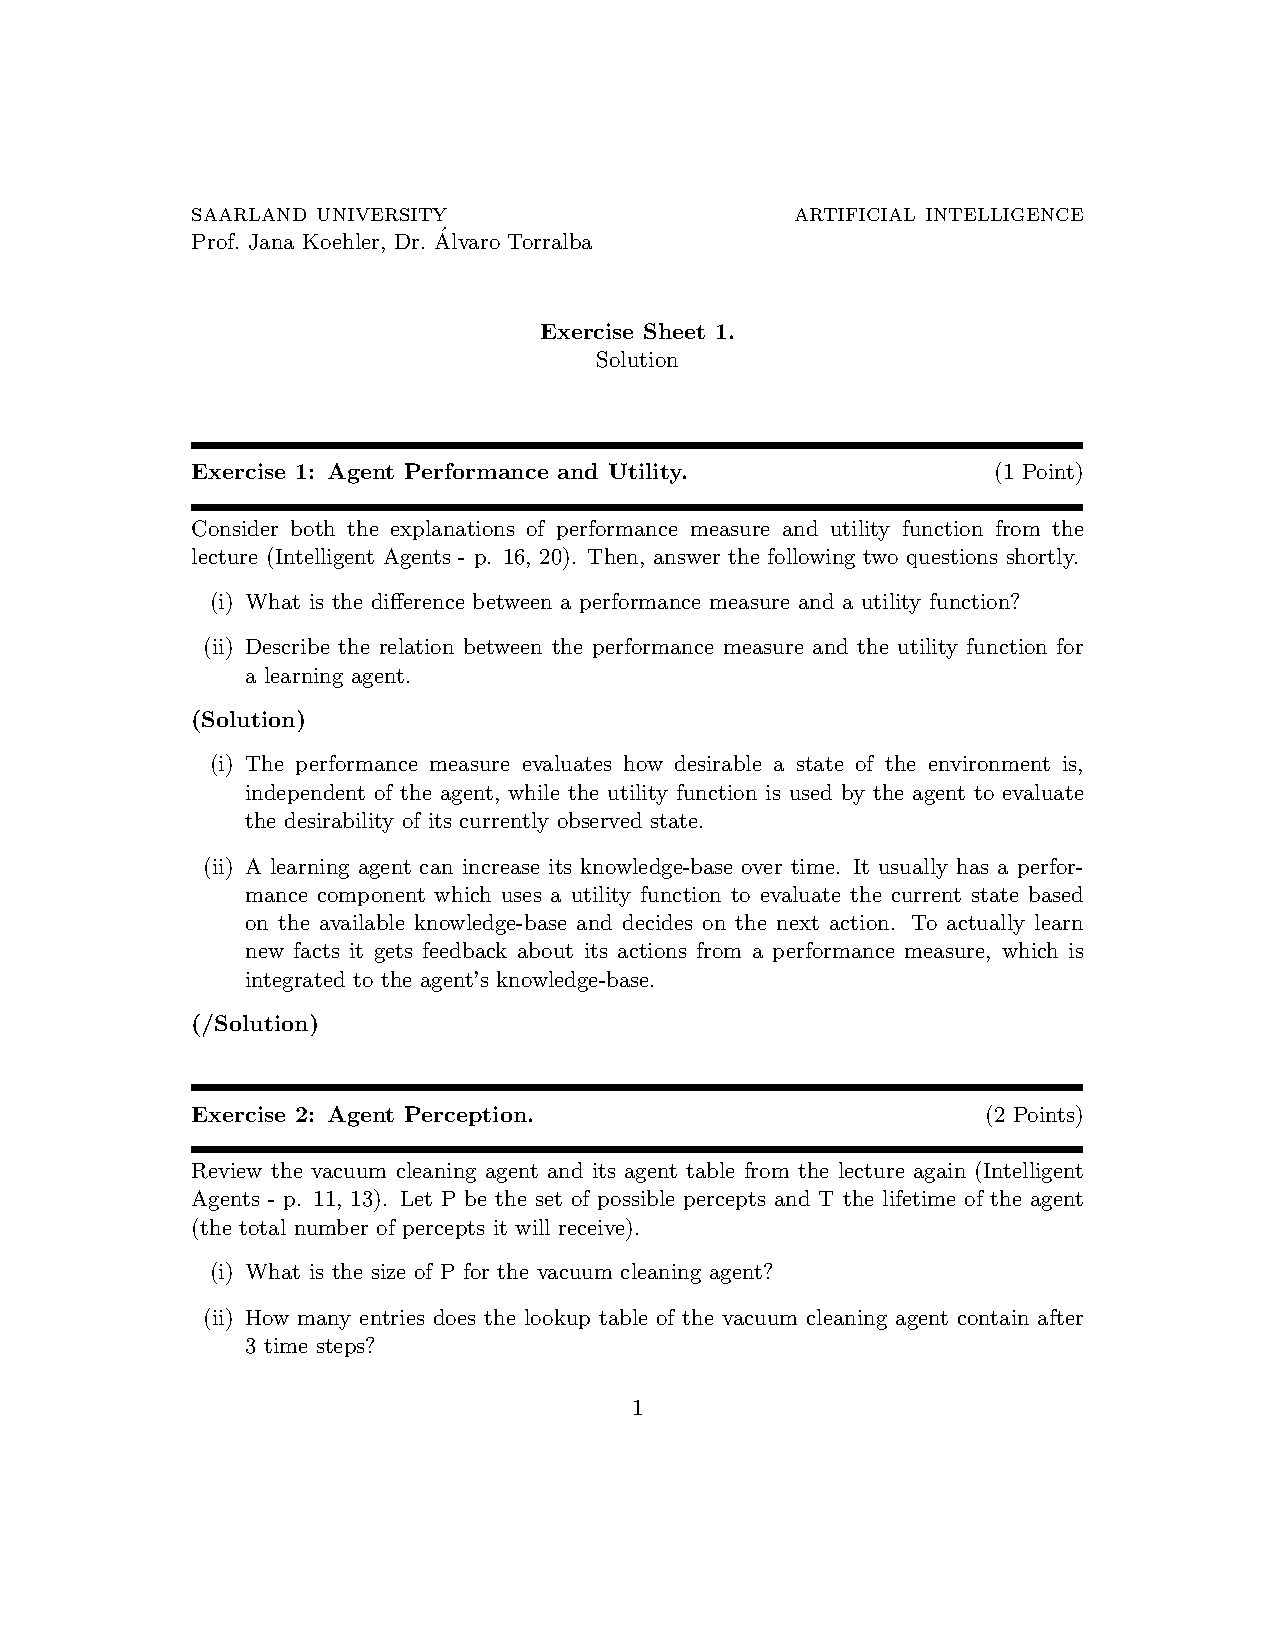
\includepdf[pages=-]{Exercise_Sheet_1_-_Solution.pdf}

\section{Sheet 1}
    \subsection{Planning a Trip from Kaiserslautern to Saarbruecken (state space, initial state, goal state, goal test and set of actions)}
    \subsection{BFS (Breath-First Search) and DLS (Depth-Limited Search)}
    \subsection{State Space}
    \subsection{IDS (Iterated-Depth Search) and UCS (Uniform-Cost Search)}
    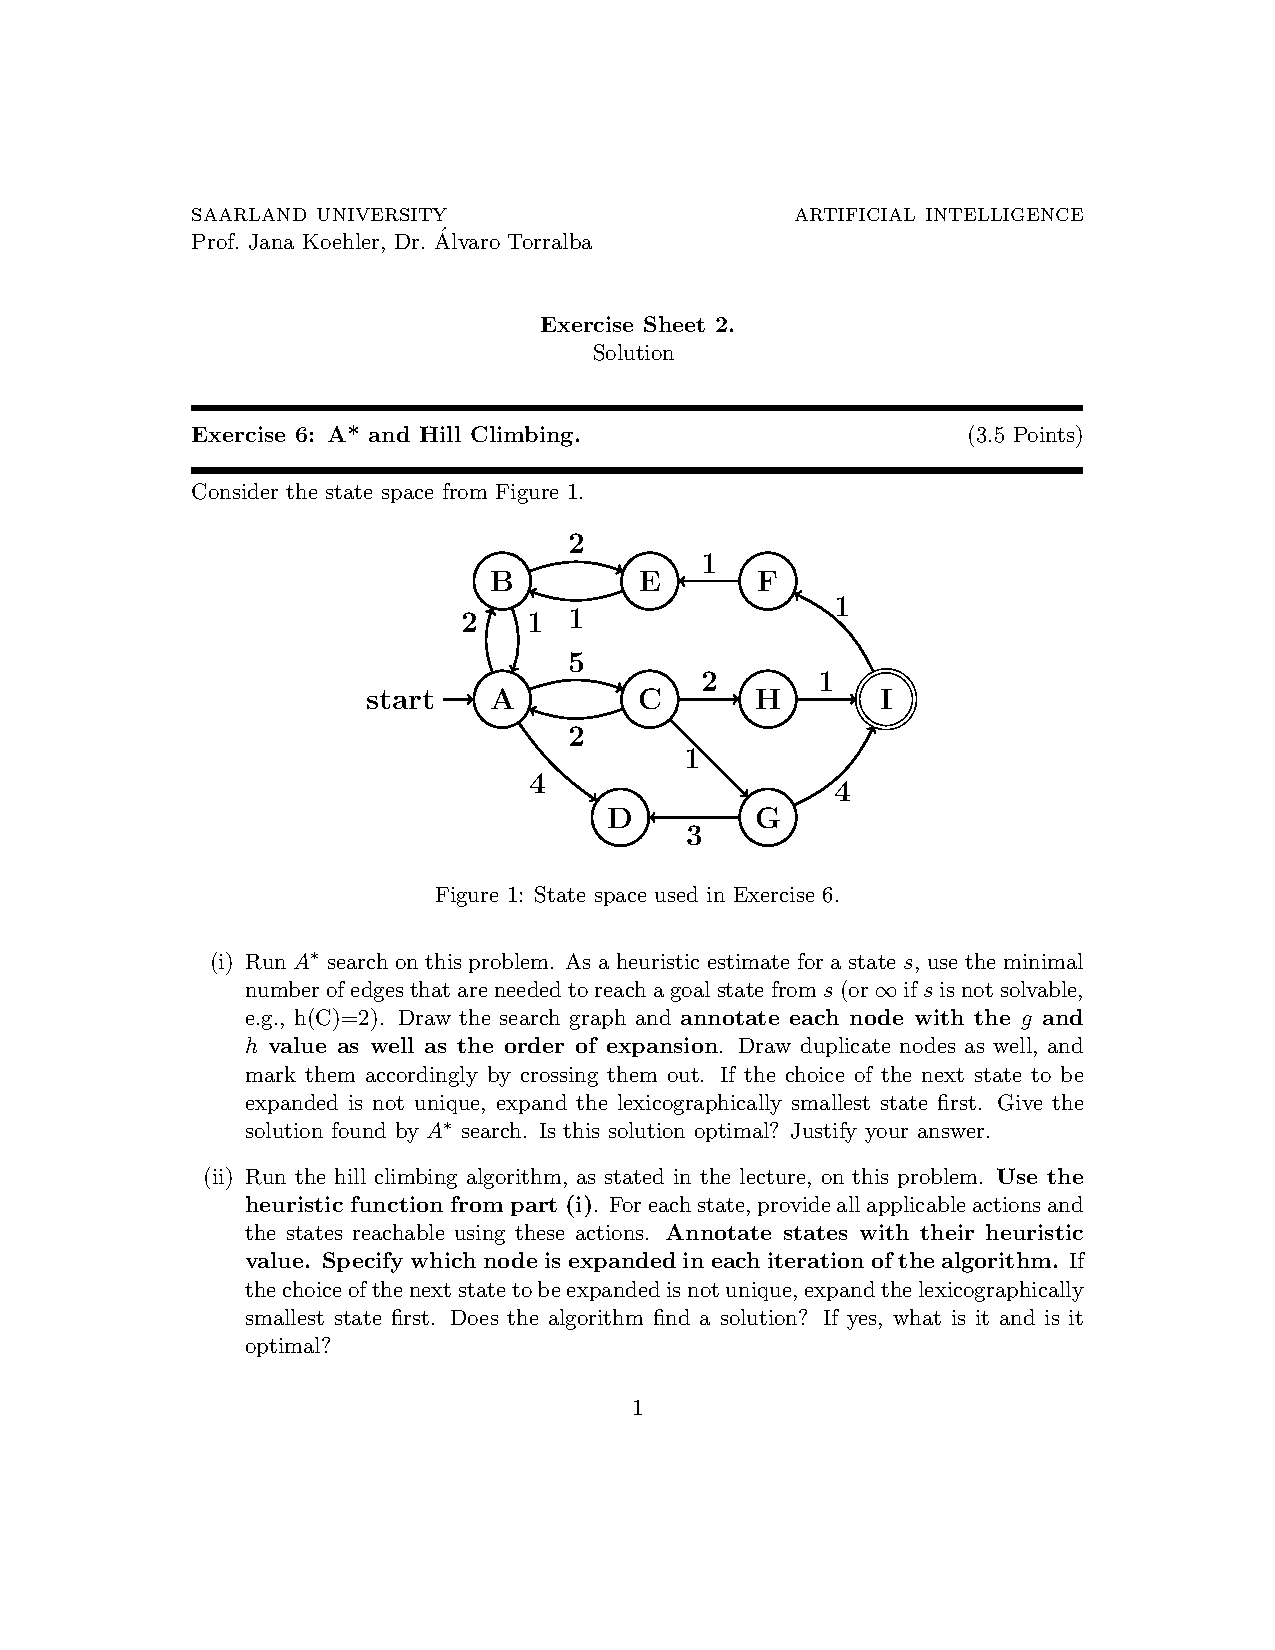
\includepdf[pages=-]{Exercise_Sheet_2_-_Solution.pdf}
    
\section{Sheet 2}
    \subsection{Heuristic Function + Manhatten Distance}
    \subsection{Ladybird in a maze (heuristic function)}
    \subsection{$A^*$}
    \subsection{UCT Flowchart}
    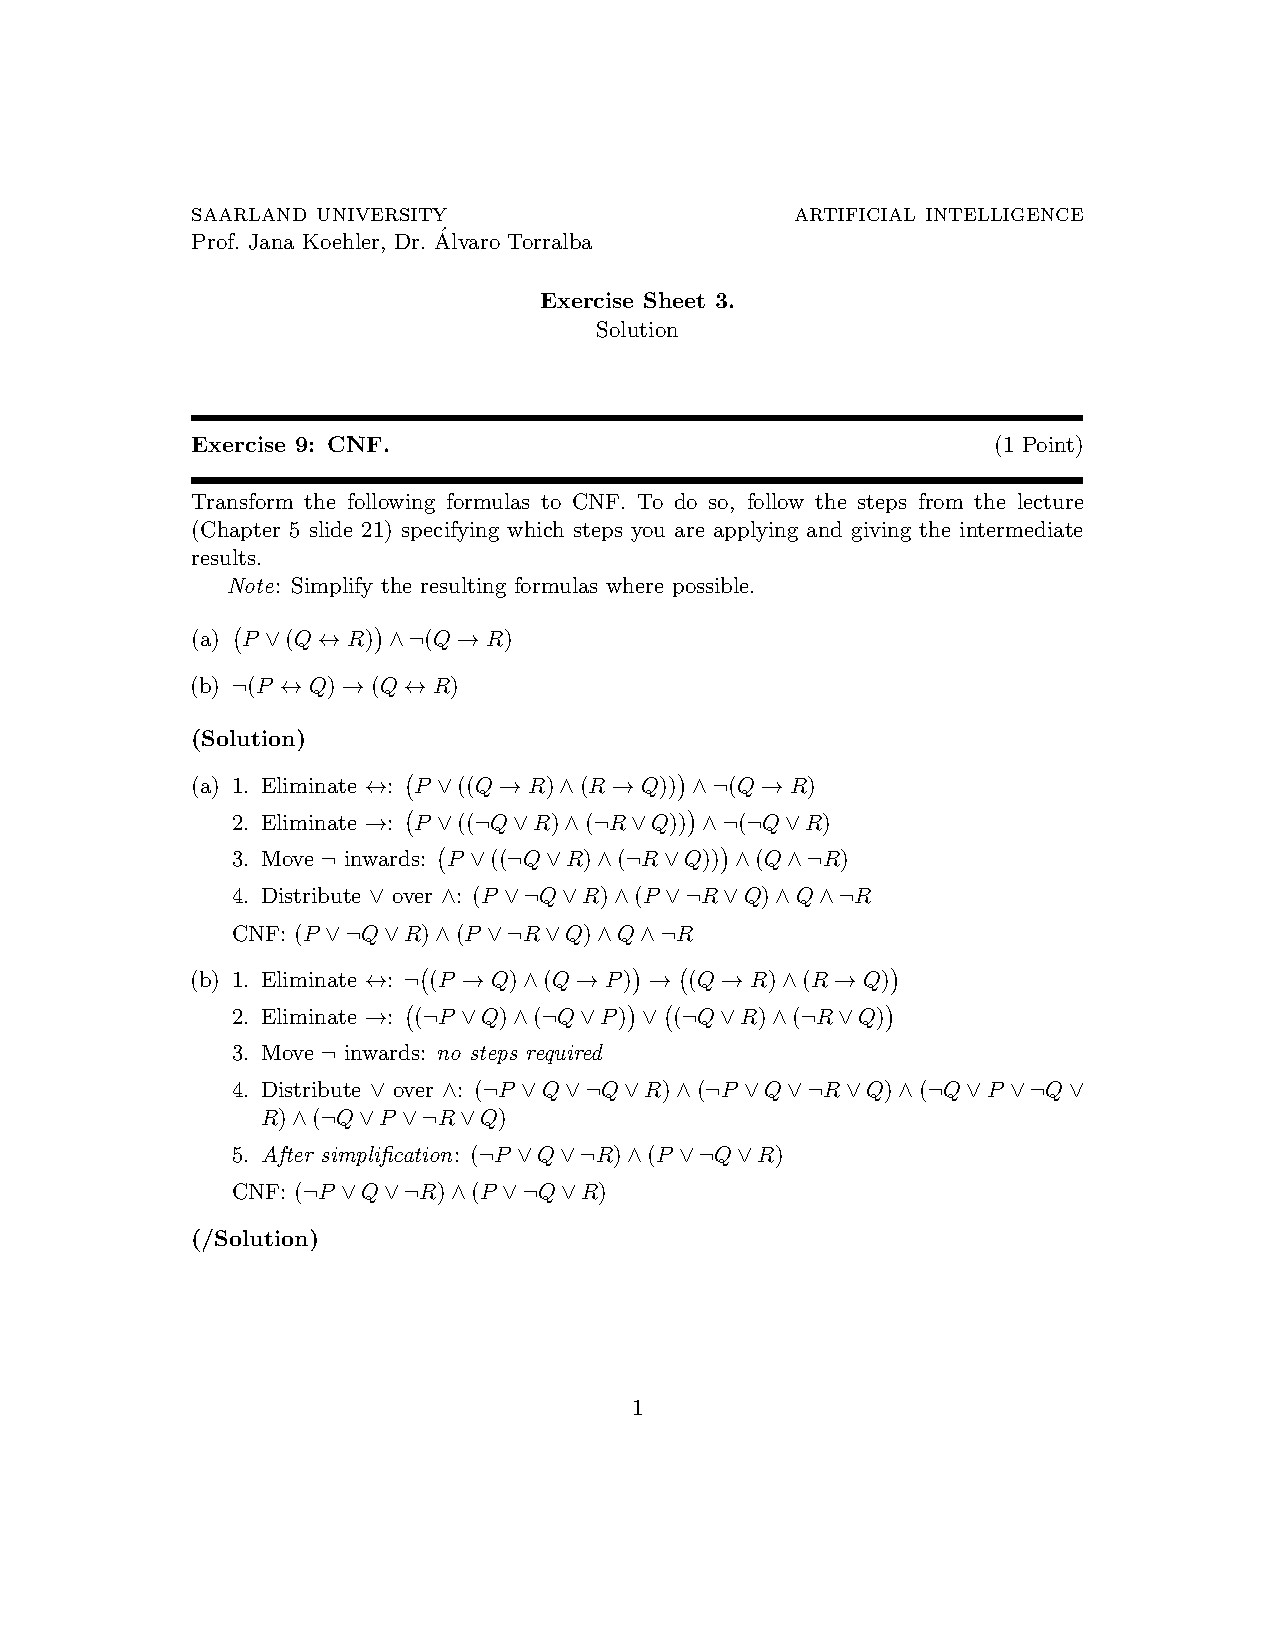
\includepdf[pages=-]{Exercise_Sheet_3_-_Solution.pdf}

\section{Sheet 3}
    \subsection{Who is guilty? (truth table)}
    \subsection{Finding Logical Formulas (DNF constructing)}
    \subsection{CNF & DNF Transformation}
    \subsection{Resolution Proof}
    \subsection{DPLL}
    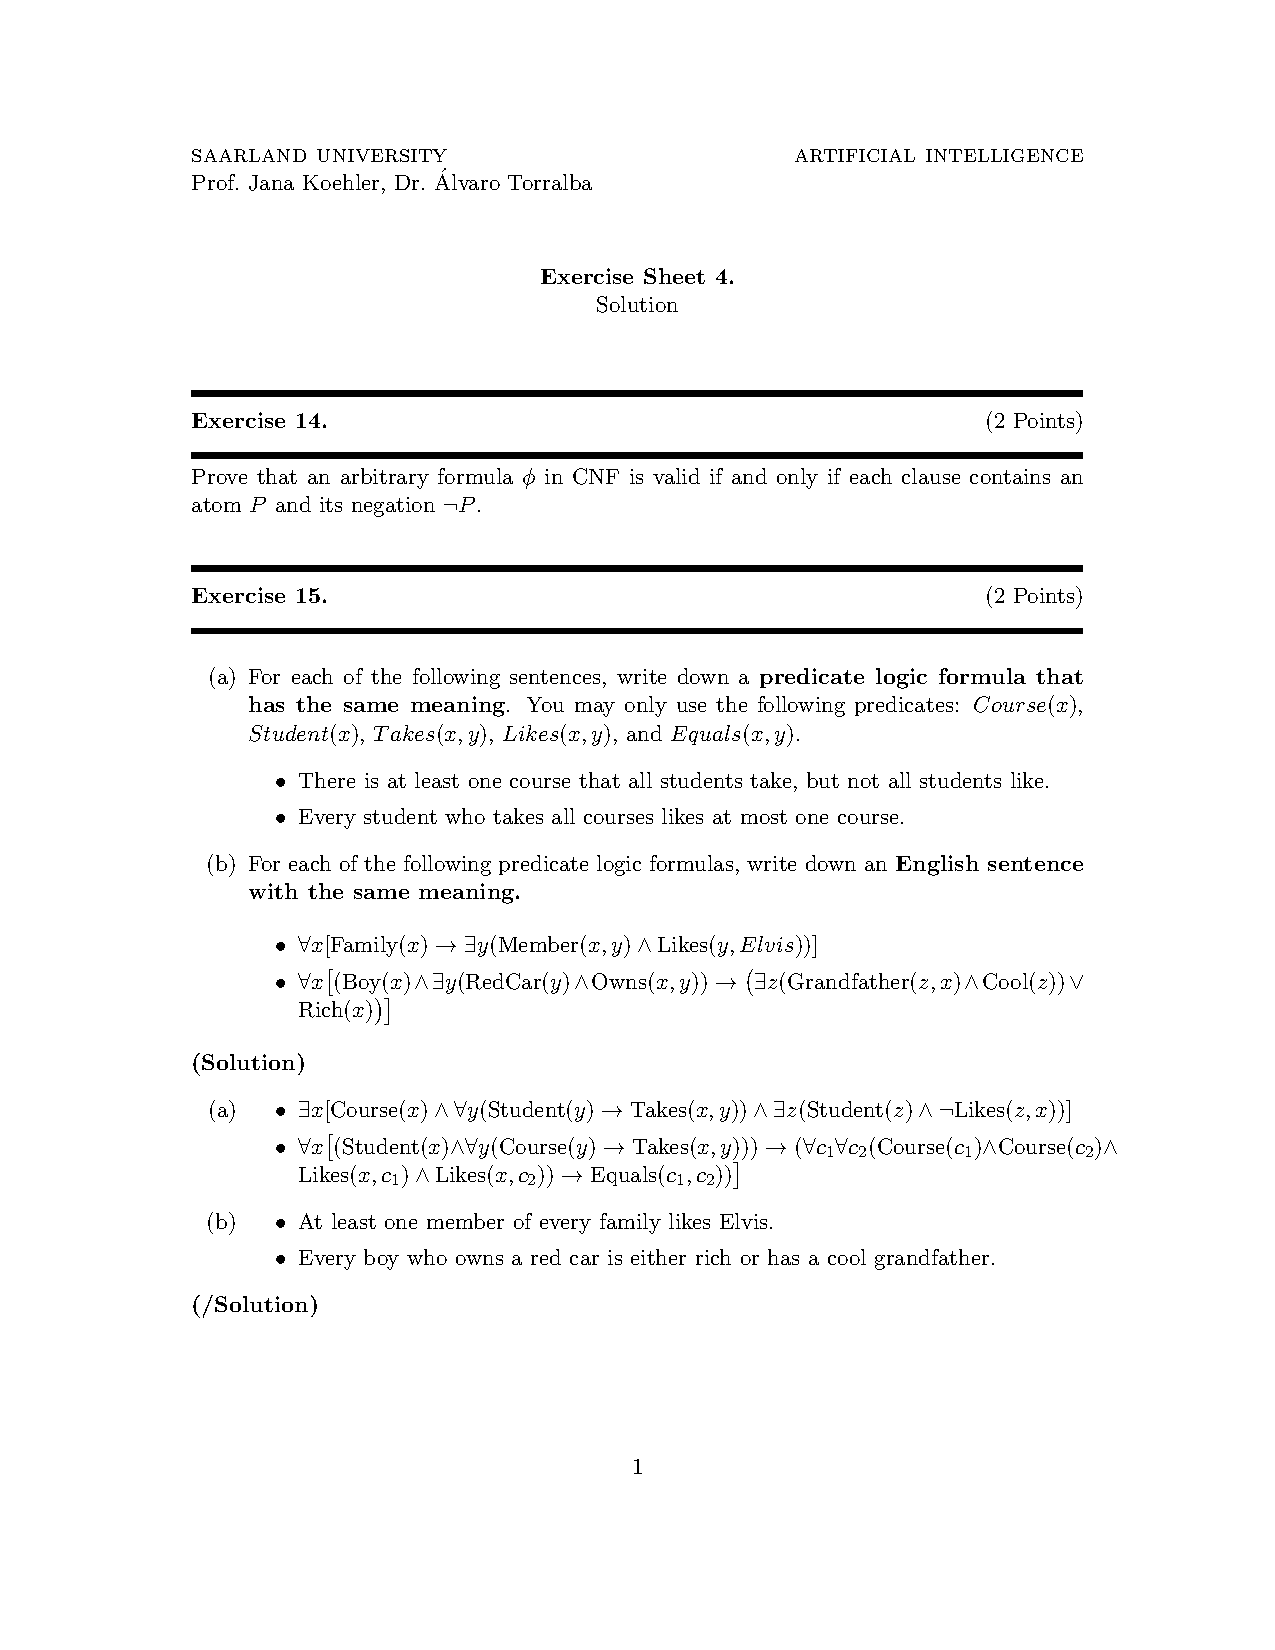
\includepdf[pages=-]{Exercise_Sheet_4_-_Solution.pdf}

\section{Sheet 4}
    \subsection{Predicate Logic Basics}
    \subsection{Normal Forms (Predicate logic formulas in CNF)}
    \subsection{Herbrand Expansion}
    \subsection{Unification}
    \subsection{PL1 Resolution (predicate logic formulas in Skolem Normal Form)}
    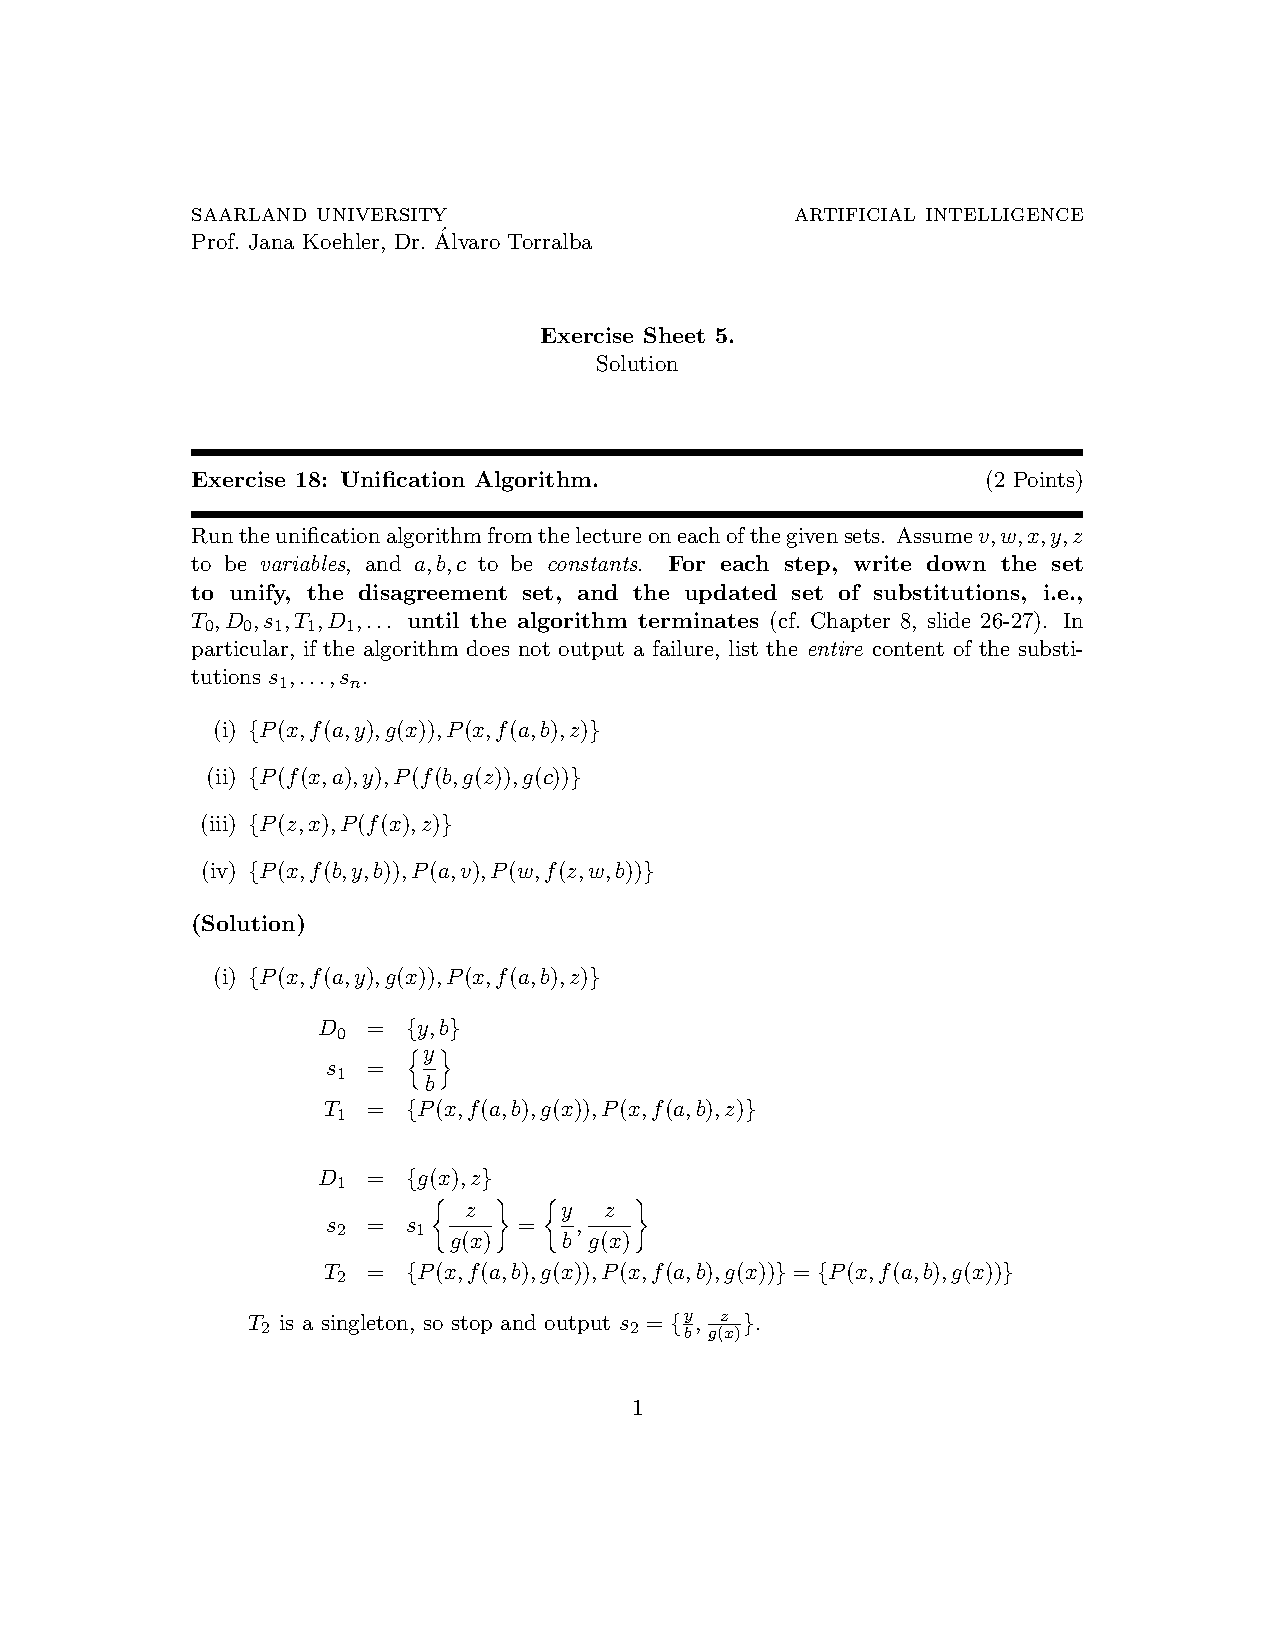
\includepdf[pages=-]{Exercise_Sheet_5_-_Solution.pdf}

\section{Sheet 5}
    \subsection{Minimax Search}
    \subsection{Alpha-Beta pruning}
    \subsection{True or False}
    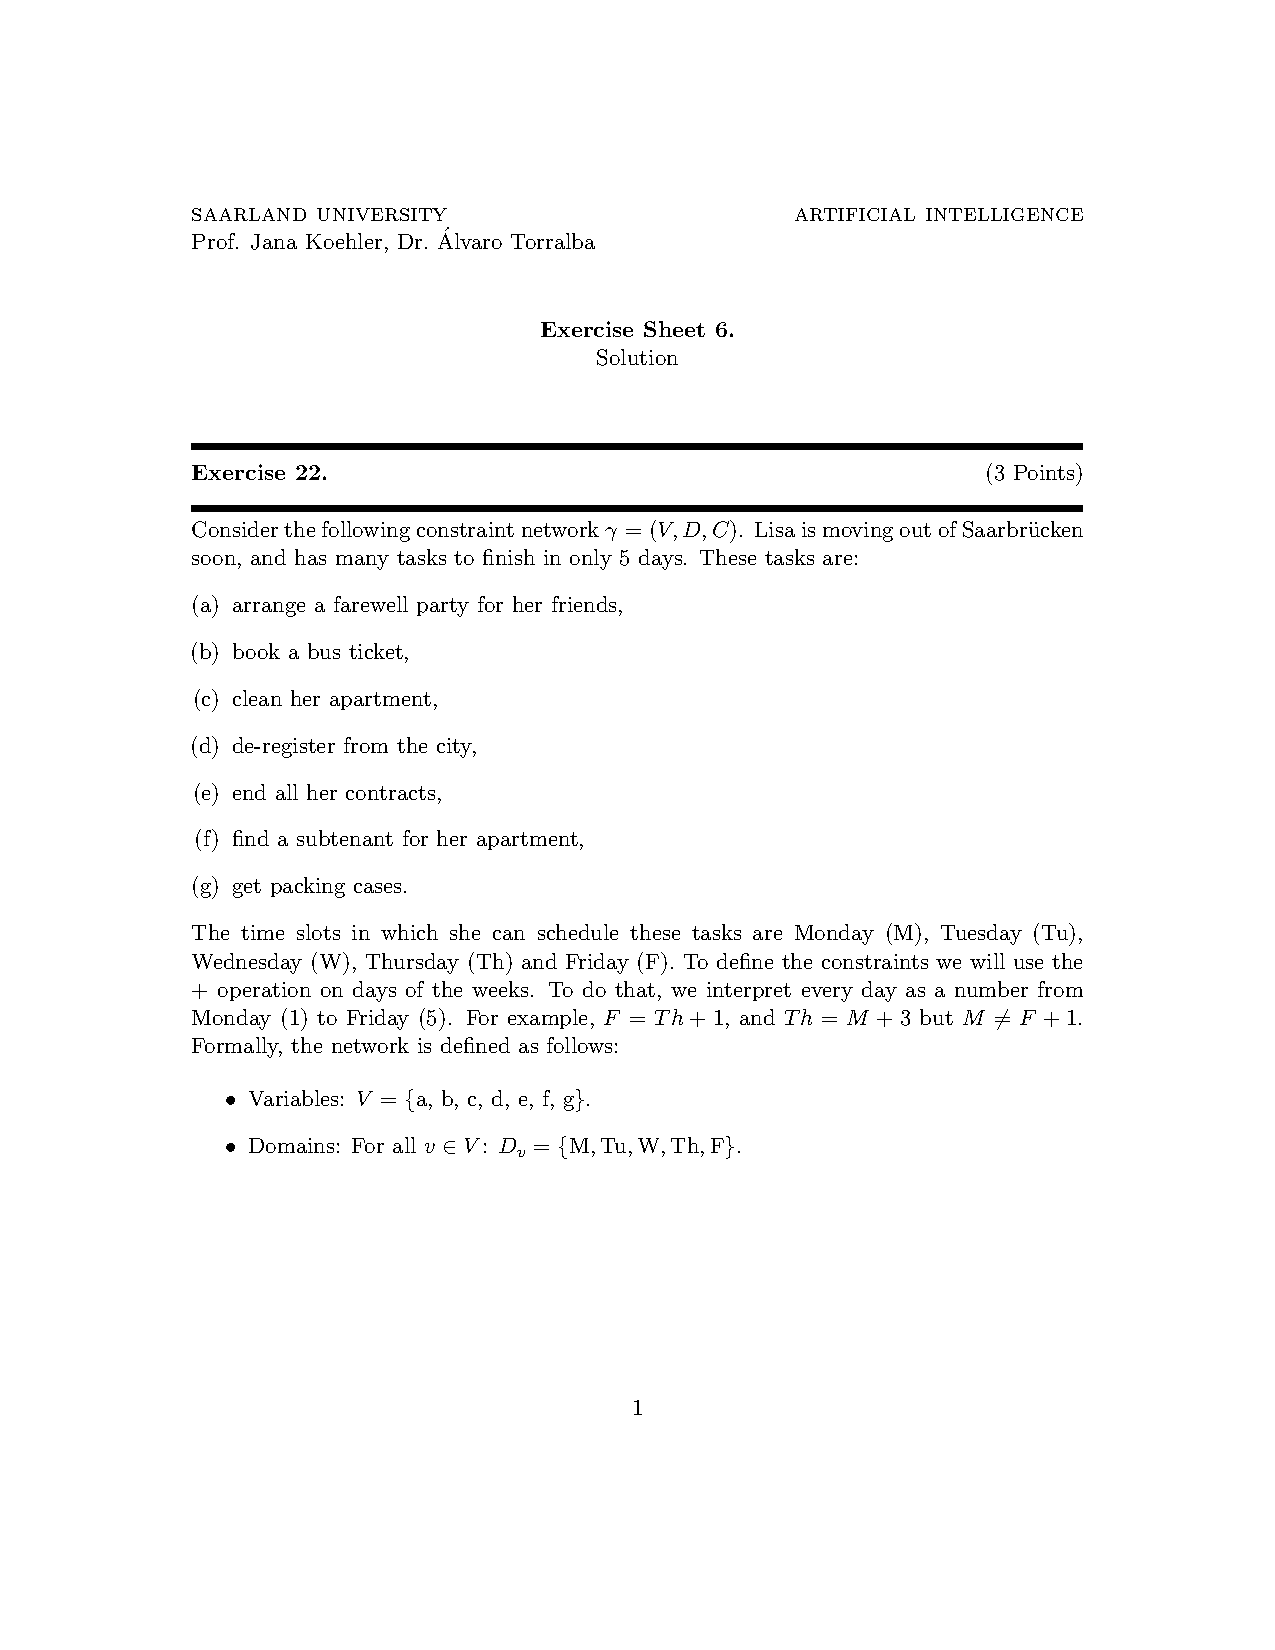
\includepdf[pages=-]{Exercise_Sheet_6_-_Solution.pdf}

\section{Sheet 6}
    \subsection{TBox Description}
    \subsection{Chaotic Metro Plan (suitable concept definition for assertions)}
    \subsection{Subsumptions ($\mathcal{ALS}$ Knowledge Base)}
    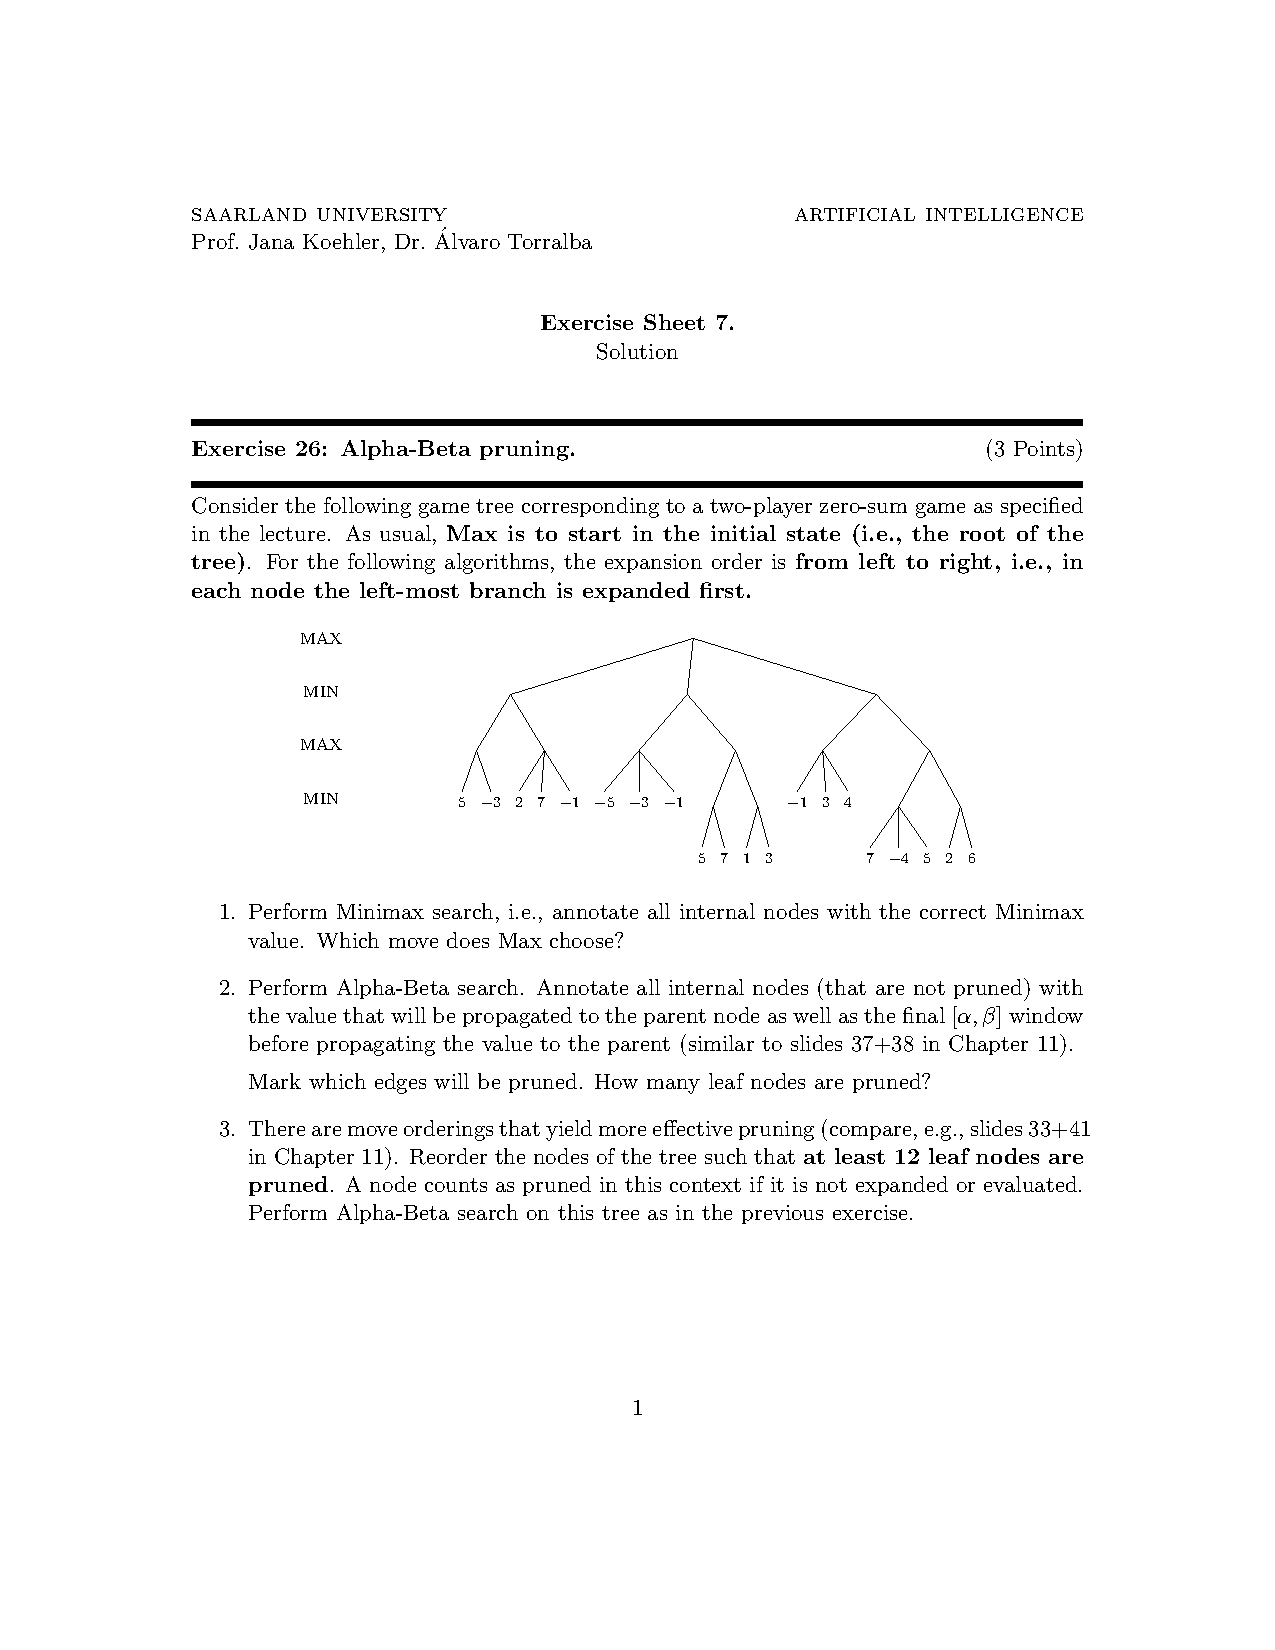
\includepdf[pages=-]{Exercise_Sheet_7_-_Solution.pdf}

\section{Sheet 7}
    \subsection{Formulating a CSP}
    \subsection{Naive Backtracking}
    \subsection{AC-3, AcyclicCG}
    \subsection{Cutset Conditioning}
    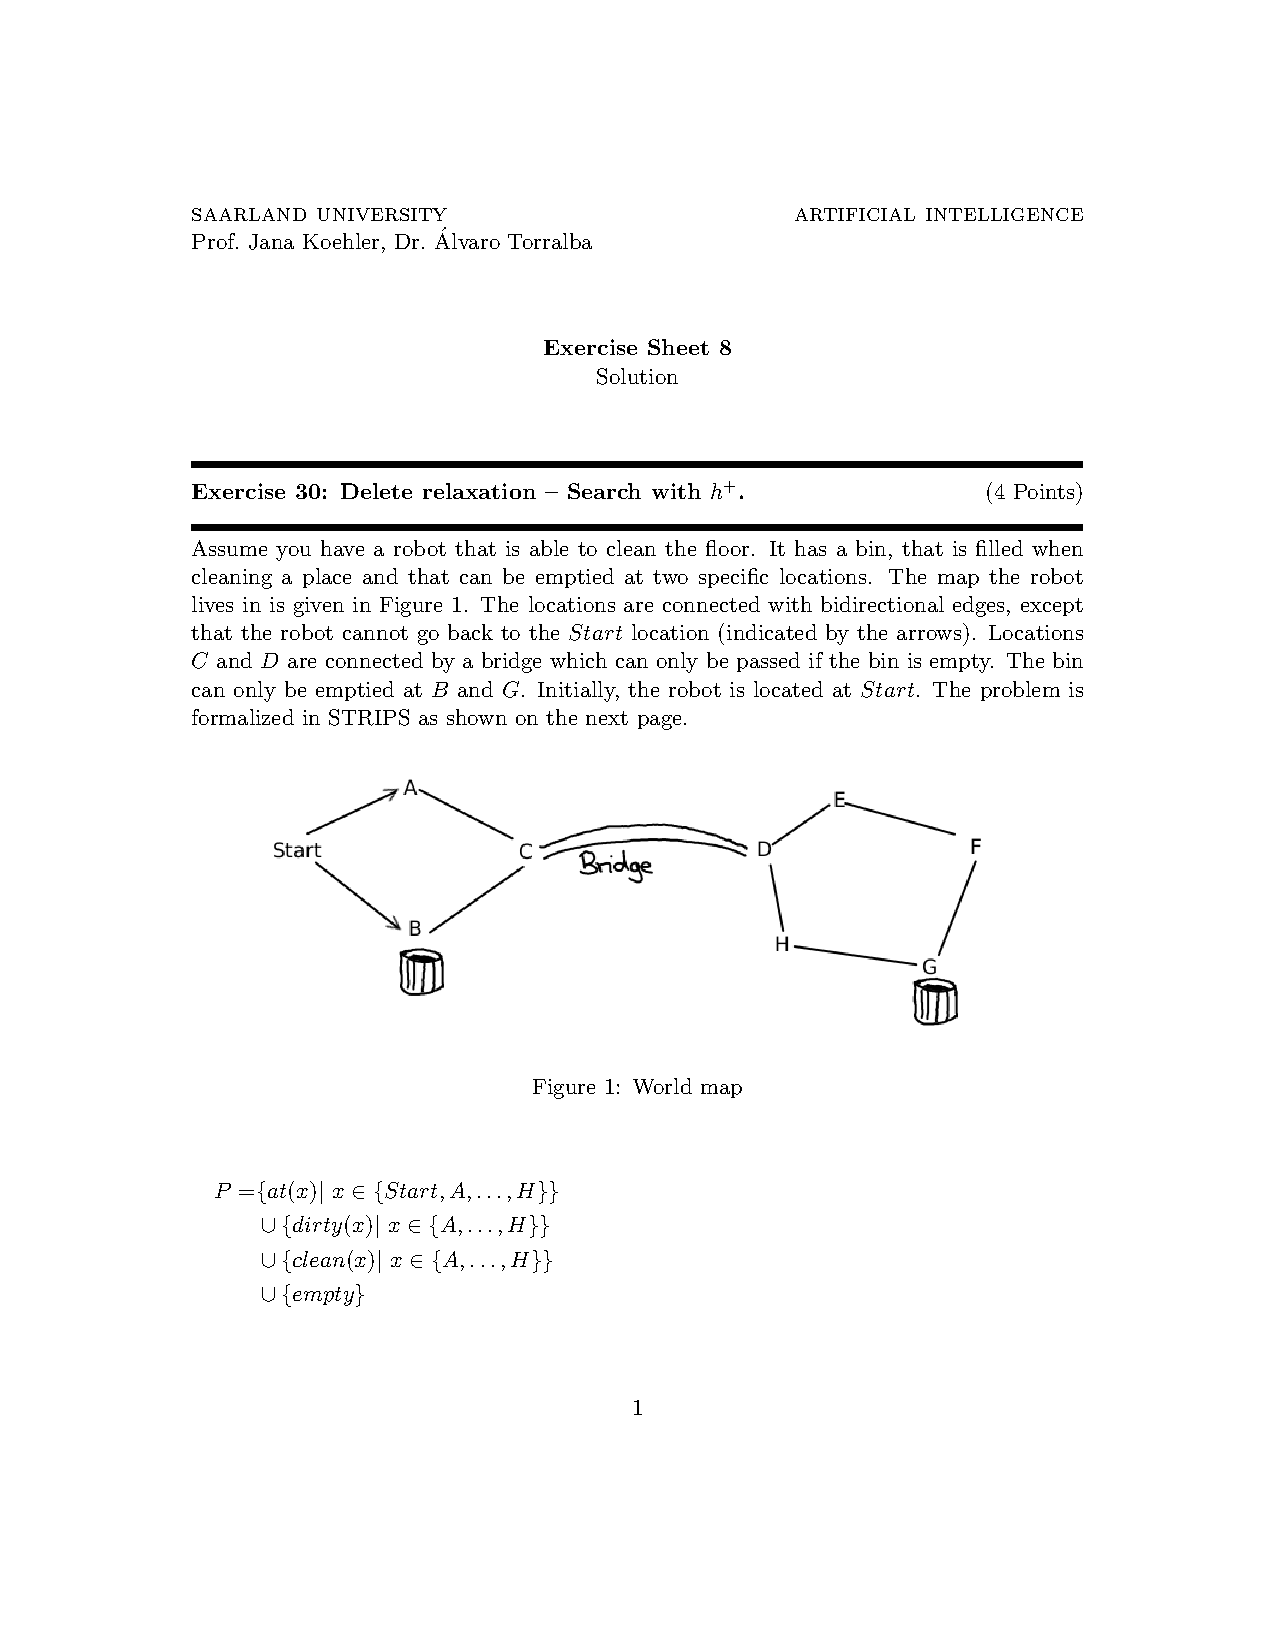
\includepdf[pages=-]{Exercise_Sheet_8_-_Solution.pdf}

\section{Sheet 8}
    \subsection{Harry's Pizza-Party (Decision-Tree-Learning algorithm)}
    \subsection{Harry's Pizza-Party Part II (Resulting tree)}
    \subsection{Fitting Functions (Ockham's razor)}
    \subsection{Spam Detection}
    \subsection{Entropy}
    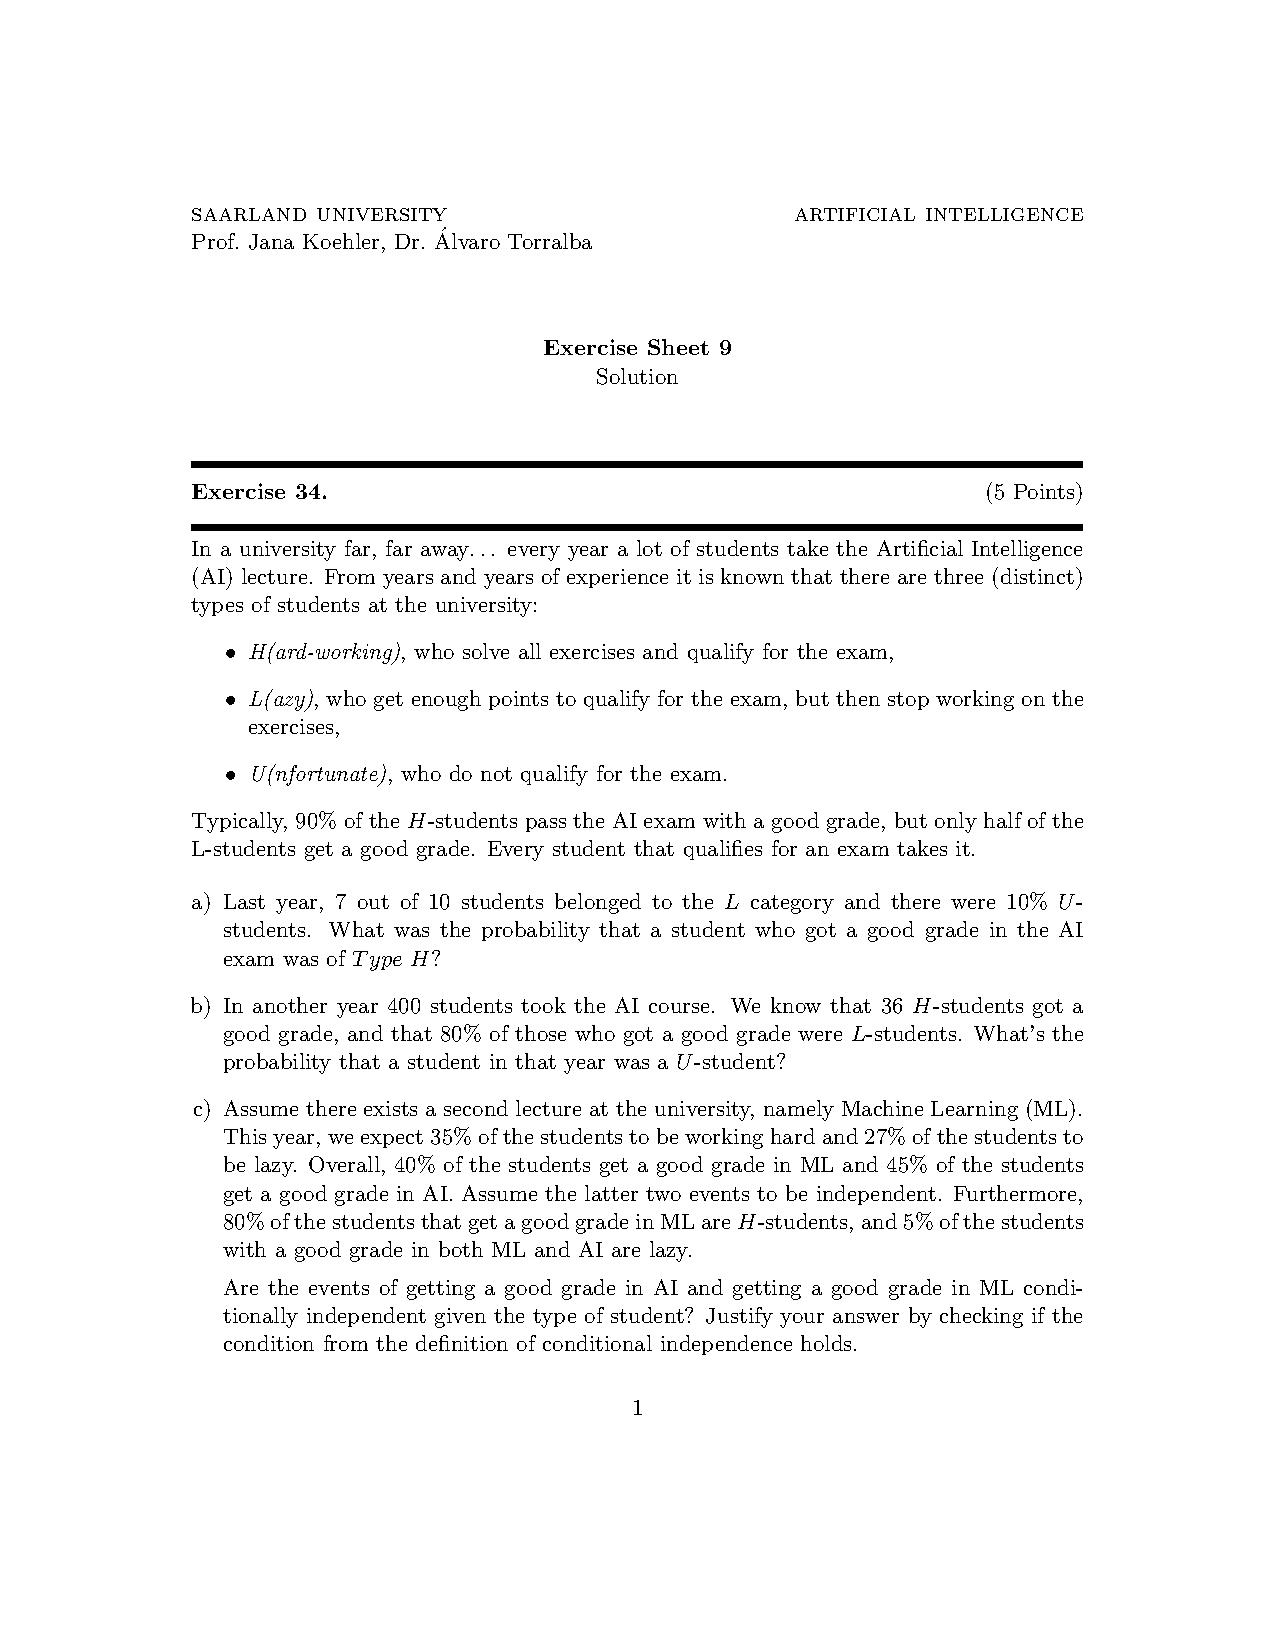
\includepdf[pages=-]{Exercise_Sheet_9_-_Solution.pdf}

\section{Sheet 10}
    \subsection{$h^{FF}$ and $h^+$}
    \subsection{True or False? (STRIPS, ...)}
    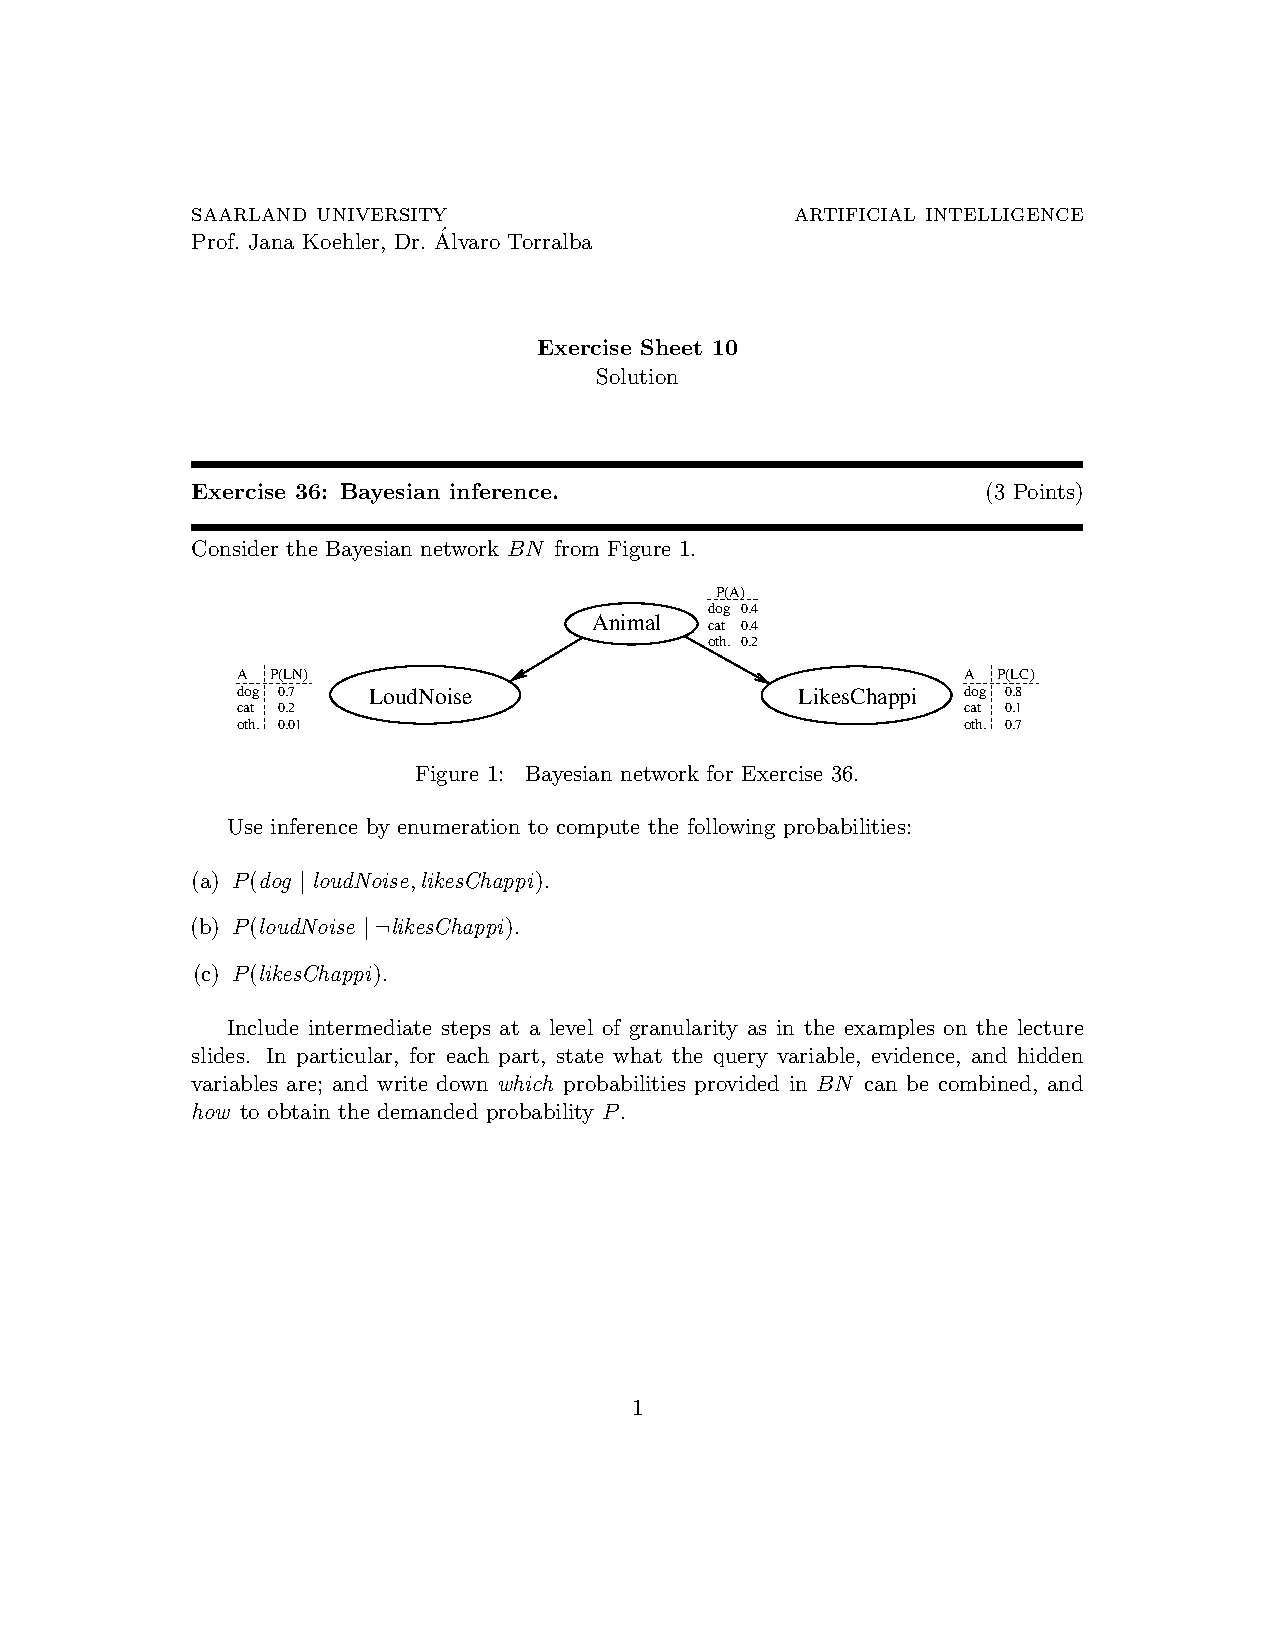
\includepdf[pages=-]{Exercise_Sheet_10_-_Solution.pdf}



\section{AI 2016}
    \subsection{Sheet 1:}
        \subsubsection{Exercise 1: UCS, $A^*$, Hill Climbing algorithm, Heuristic, Iterative DFS}
        \subsubsection{Exercise 2: Vacuum Cleaner (Heuristic), }
        \subsubsection{Exercise 3: DFS, Iterative-Deepening search}
    \subsection{Sheet 2:}
        \subsubsection{Exercise 4: Tic-Tac-Toe (Minimax), Evaluation Function}
        \subsubsection{Exercise 5: Minimax search, Alpha-Beta search, Pruning}
        \subsubsection{Exercise 6: Naive Backtracking, Variable Ordering}
        \subsubsection{Exercise 7: Crossword Puzzle, Specify variable domains and constraints}
    \subsection{Sheet 3:}
        \subsubsection{Exercise 8: Naive Backtracking, Constraint Network, CSP Problem}
        \subsubsection{Exercise 9: Constraint Network, AC-3}
        \subsubsection{Exercise 10: Constraint Network, AcyclicCG, BacktrackingWithInference}
        \subsubsection{Exercise 11: Constraint Network, Optimal (minimal) Cutset, Cutset Conditioning algorithm, AcyclicCG}
    \subsection{Sheet 4:}
        \subsubsection{Exercise 13: Transform to CNF}
        \subsubsection{Exercise 14: Use resolution that CNF formulas are unsatisfiable}
        \subsubsection{Exercise 15: DPLL}
\newpage
    \subsection{Sheet 5:}
        \subsubsection{Exercise 18: DPLL with clause learning}
        \subsubsection{Exercise 19: Predicate Logic Formula}
        \subsubsection{Exercise 20: Transform Predicate Logic Formulas into Clausal Normal Form}
    \subsection{Sheet 6:}
        \subsubsection{Exercise 21: Unification algorithm}
        \subsubsection{Exercise 22: Predicate Logic Formulas in Skolem Normal Form}
        \subsubsection{Exercise 23: Skolem Normal Form, Clausal Normal Form, Binary PL1 Resolution}
    \subsection{Sheet 7:}
        \subsubsection{Exercise 25: Planning Task, STRIPS formalization}
        \subsubsection{Exercise 26: Planning Task, STRIPS formalization}
        \subsubsection{Exercise 27: Planning Task, STRIPS formalization, road map, search on tree}
    \subsection{Sheet 8:}
        \subsubsection{Exercise 29: Blocksworld Problem, $h^{FF}$, $A^*$, $h^+$}
        \subsubsection{Exercise 30: Blocksworld problem, STRIPS, $h^{add}$}
    \subsection{Sheet 9:}
        \subsubsection{Exercise 1: Model an Indoor Soccer-Team Ontology in RDF}
        \subsubsection{Exercise 2: Taxonomy}
        \subsubsection{Exercise 3: Roles}
    \subsection{Sheet 10:}
        \subsubsection{Exercise 1: OWL - Preparation}
        \subsubsection{Exercise 2: OWL - Ontology Browsing}
        \subsubsection{Exercise 3: Production Systems}
    
        
    
    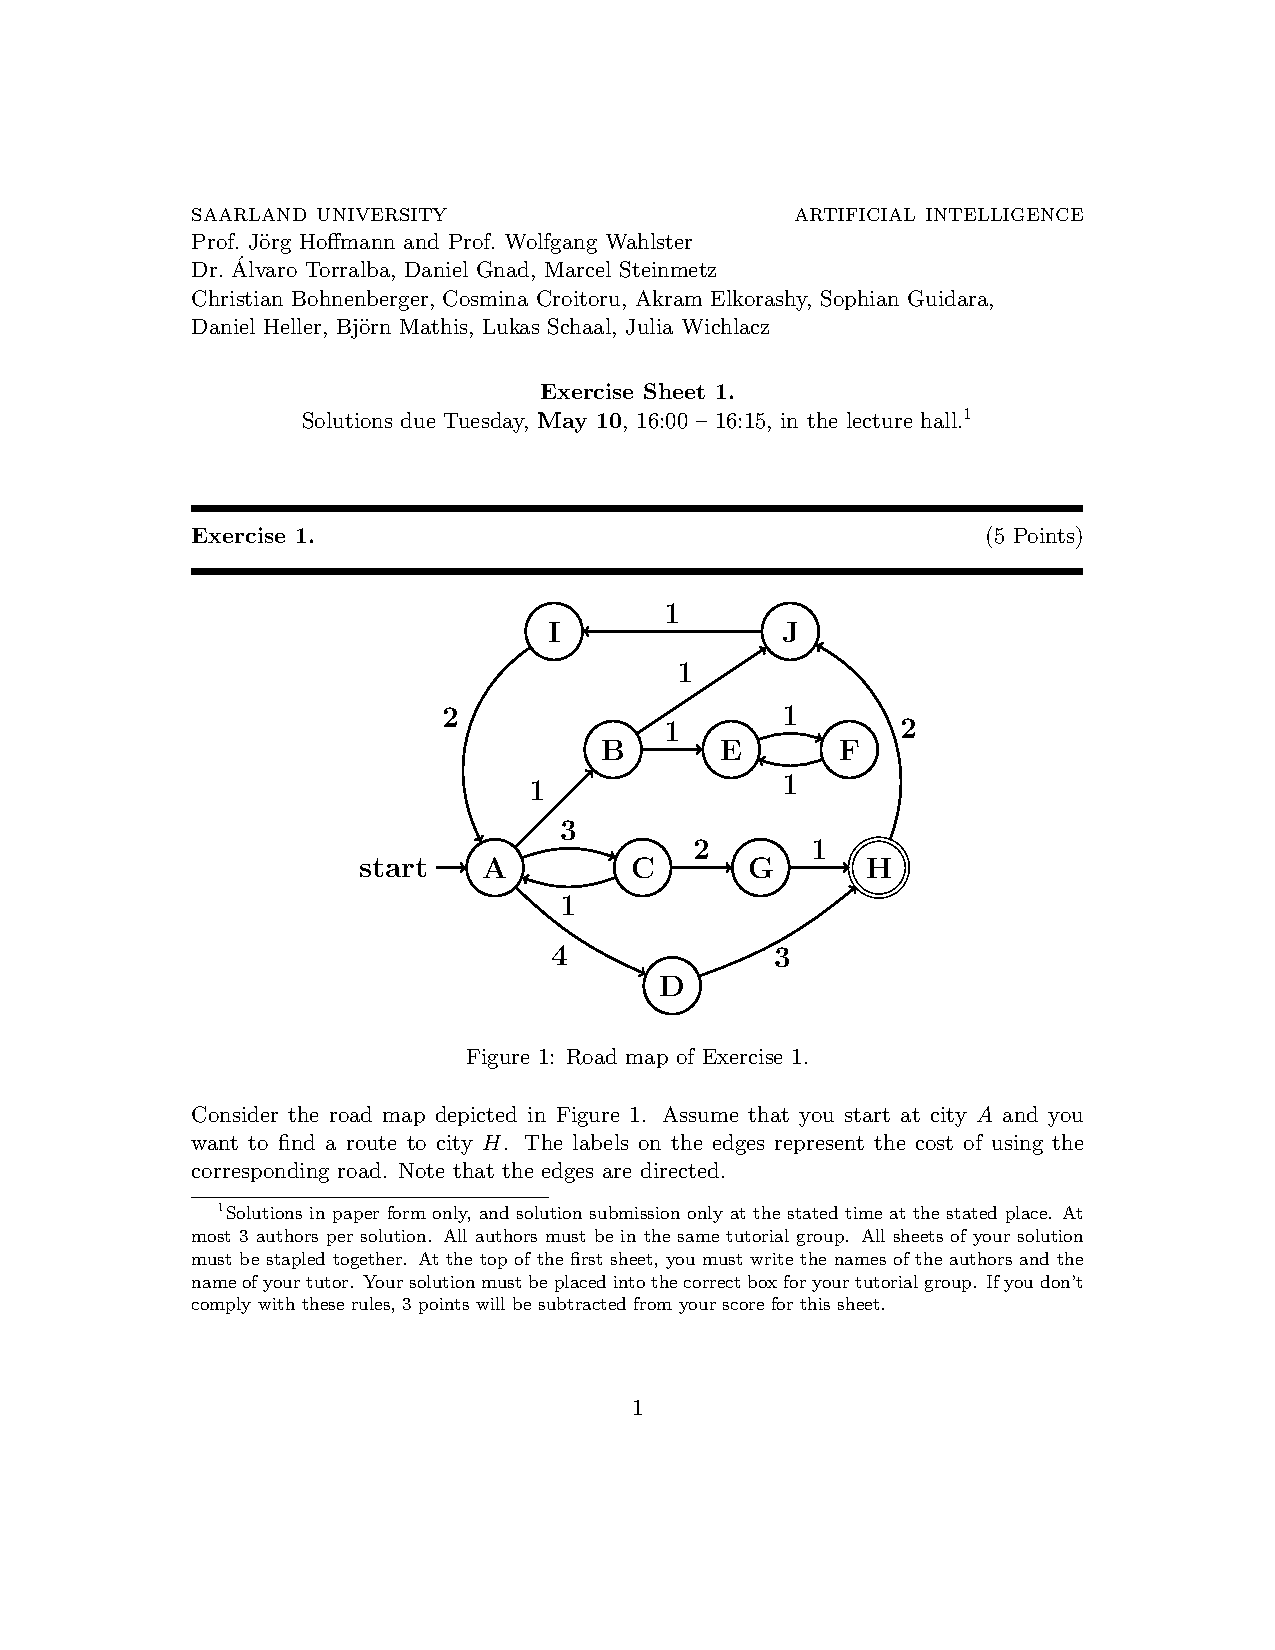
\includepdf[pages=-,nup=2x2]{Old/ai16_sheet01_solution.pdf}
    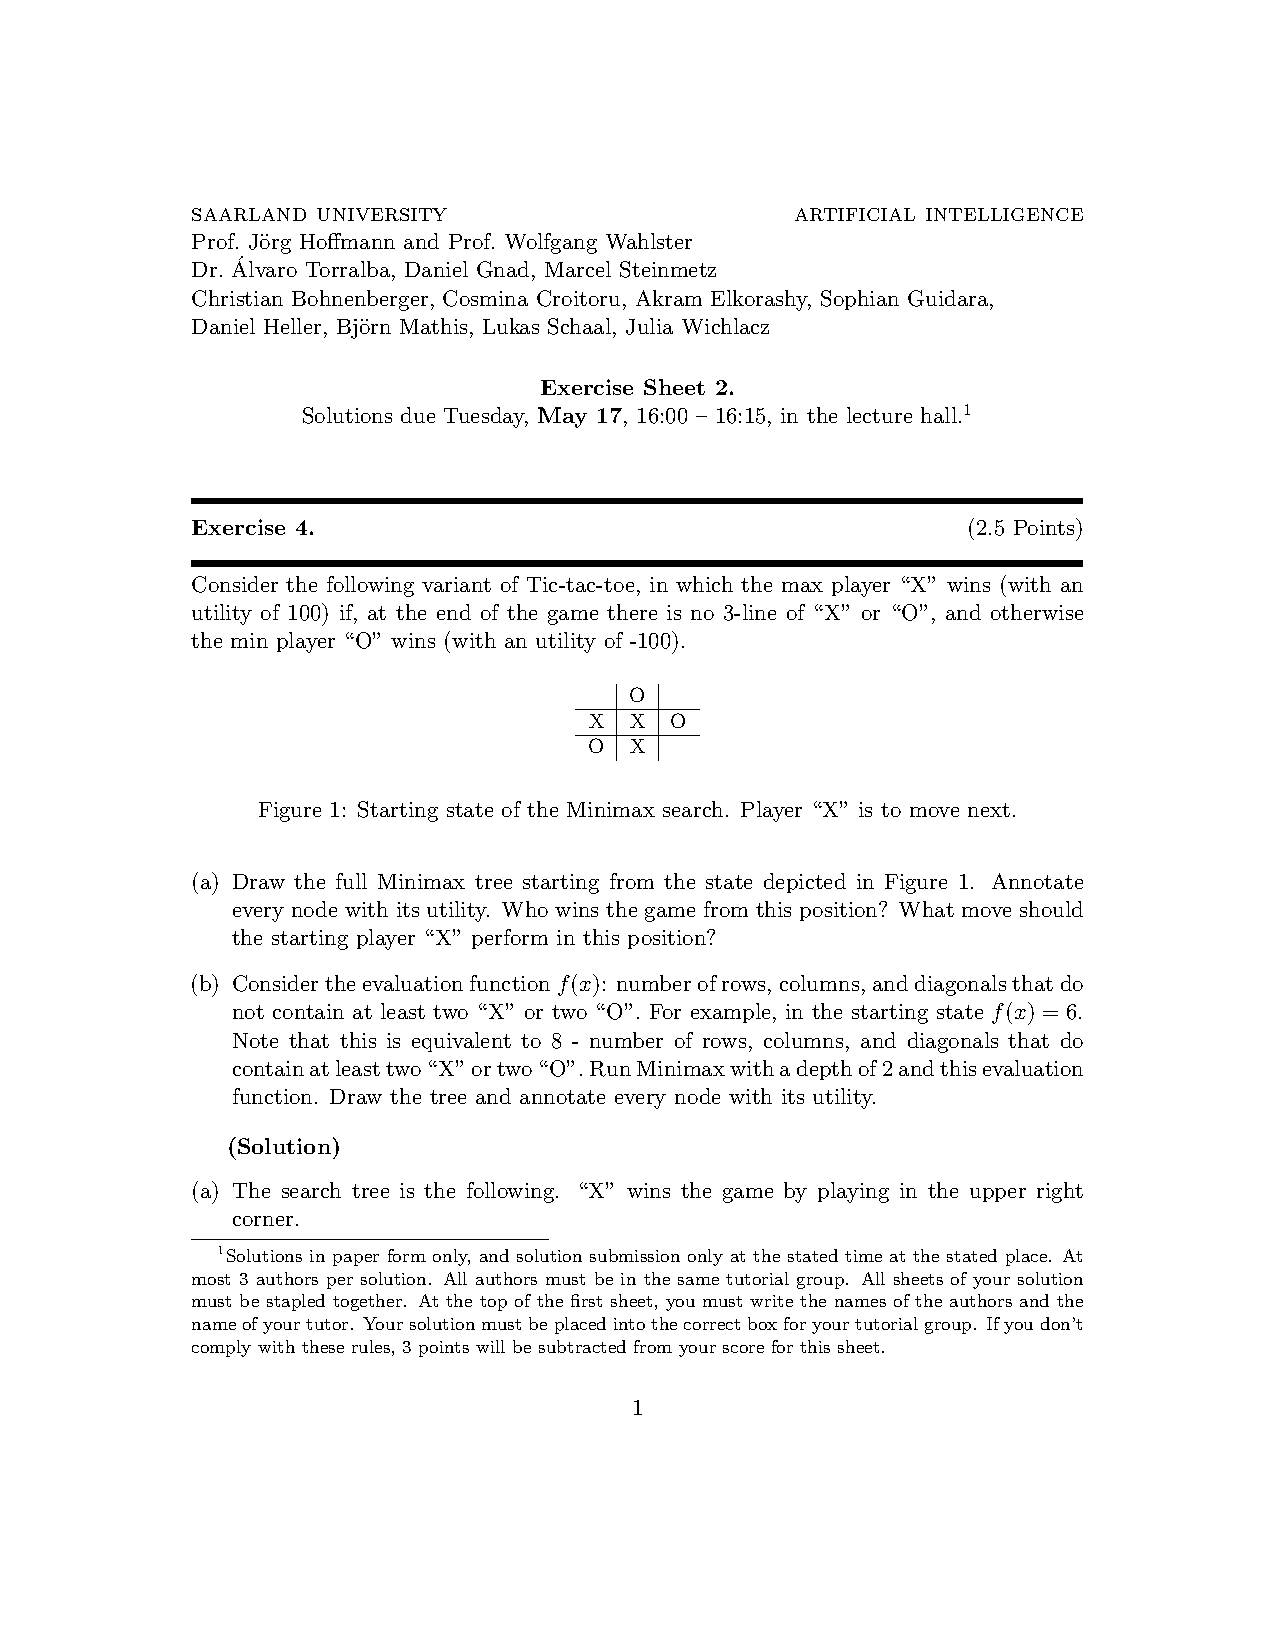
\includepdf[pages=-,nup=2x2]{Old/ai16_sheet02_solution.pdf}
    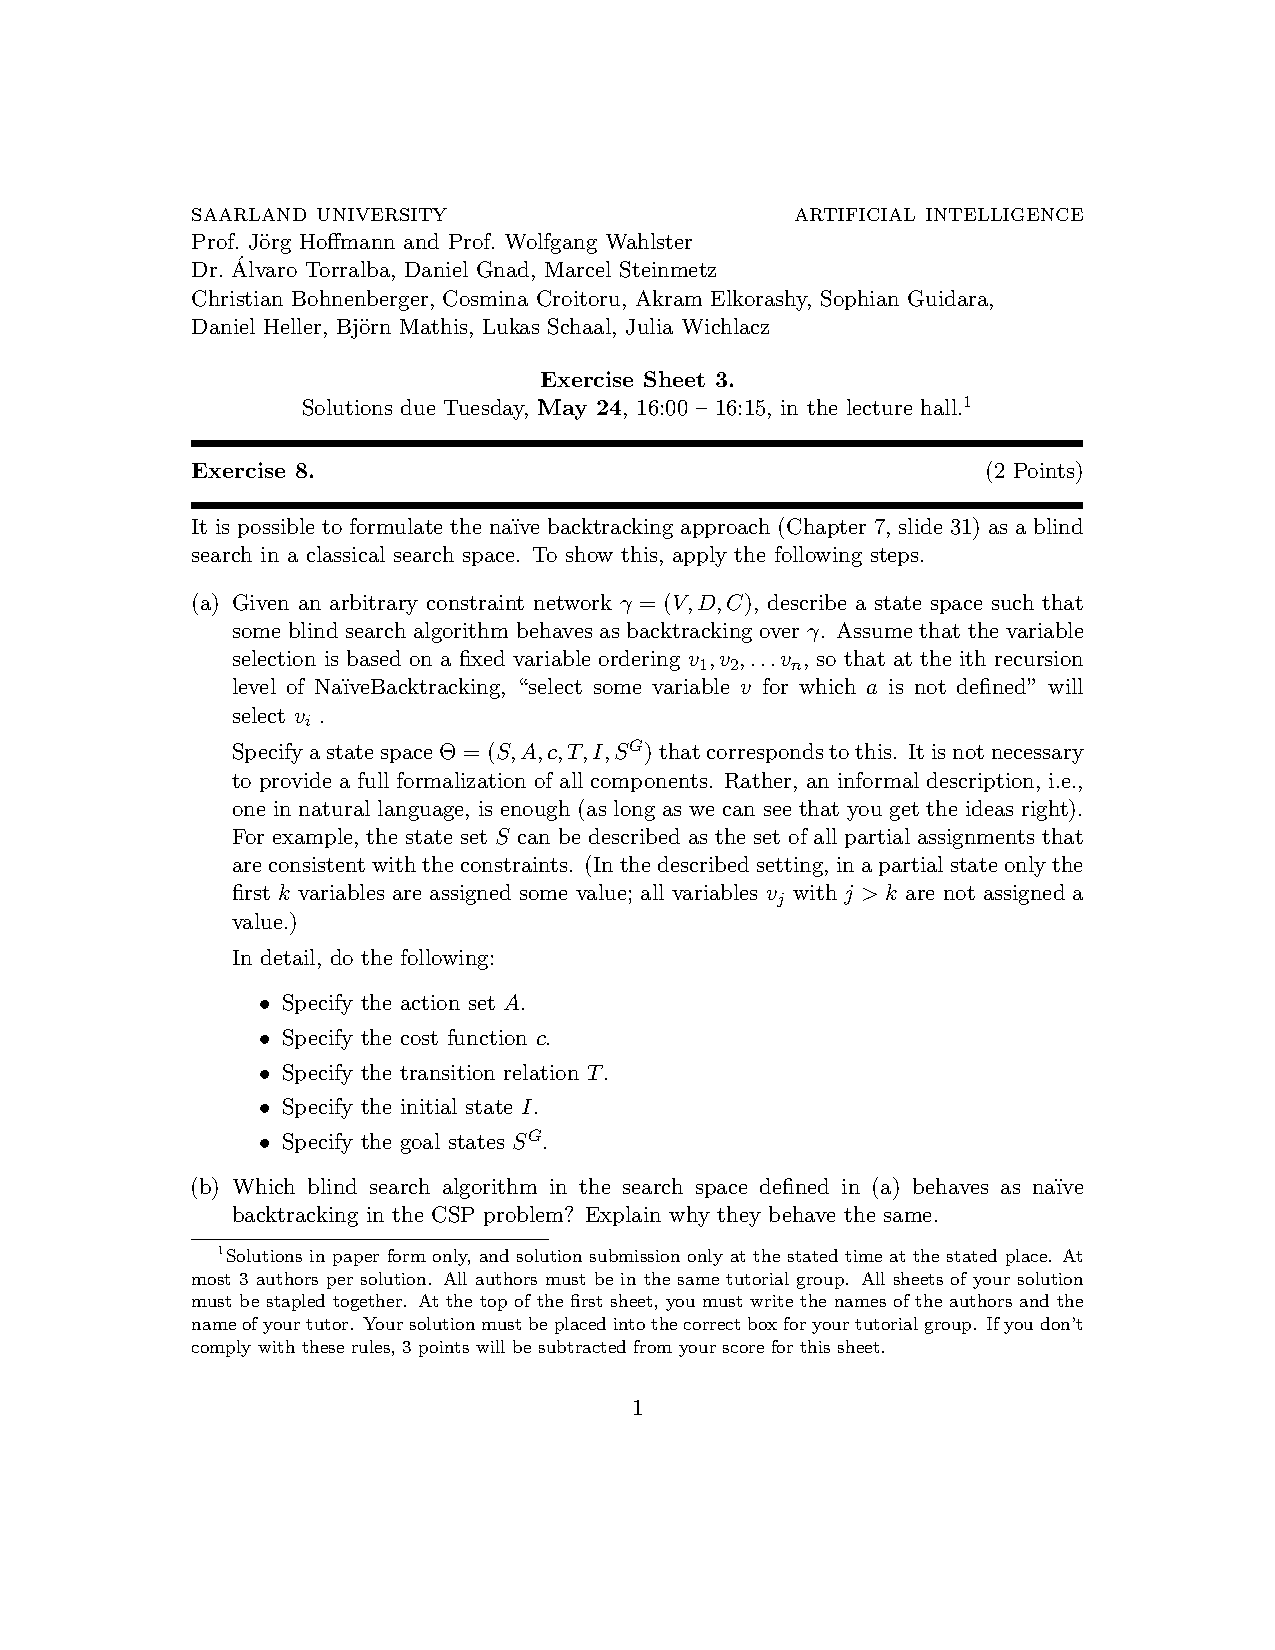
\includepdf[pages=-,nup=2x2]{Old/ai16_sheet03_solution.pdf}
    
    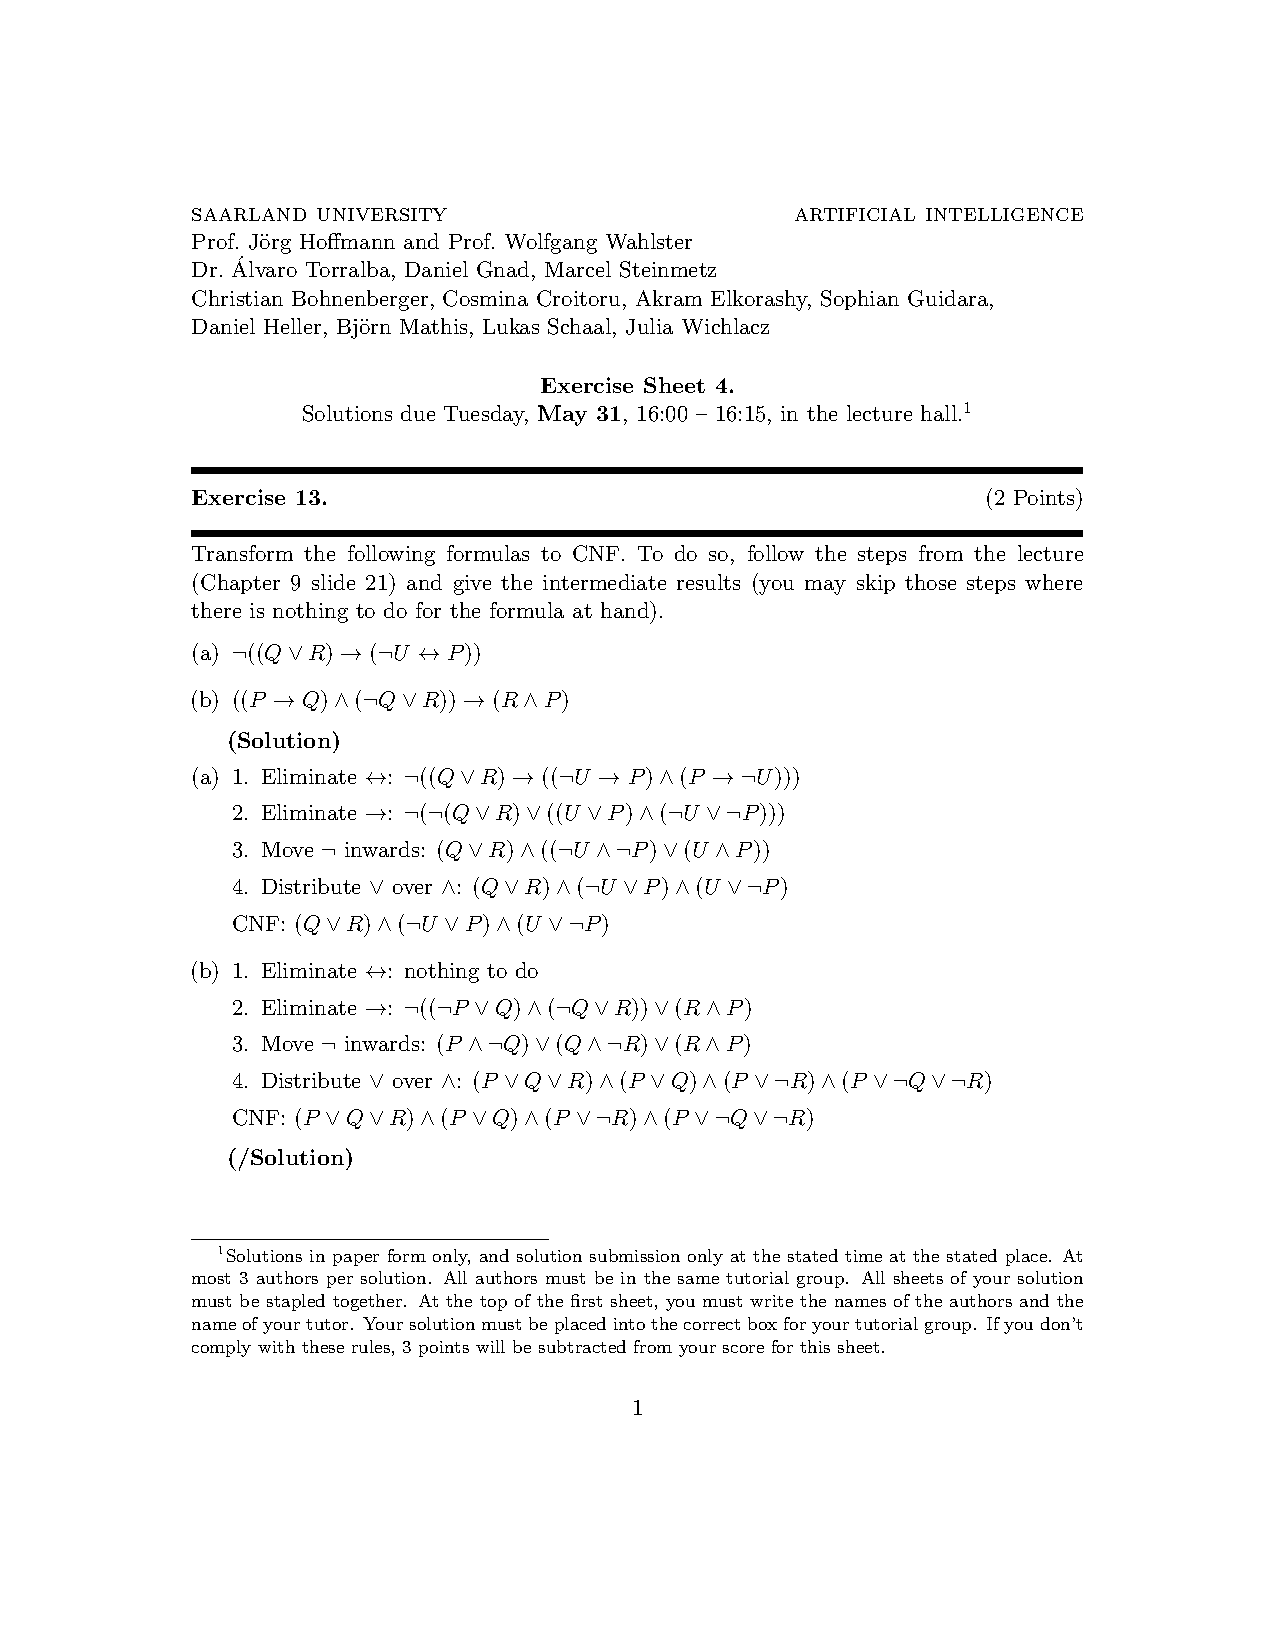
\includepdf[pages=-,nup=2x2]{Old/ai16_sheet04_solution.pdf}
    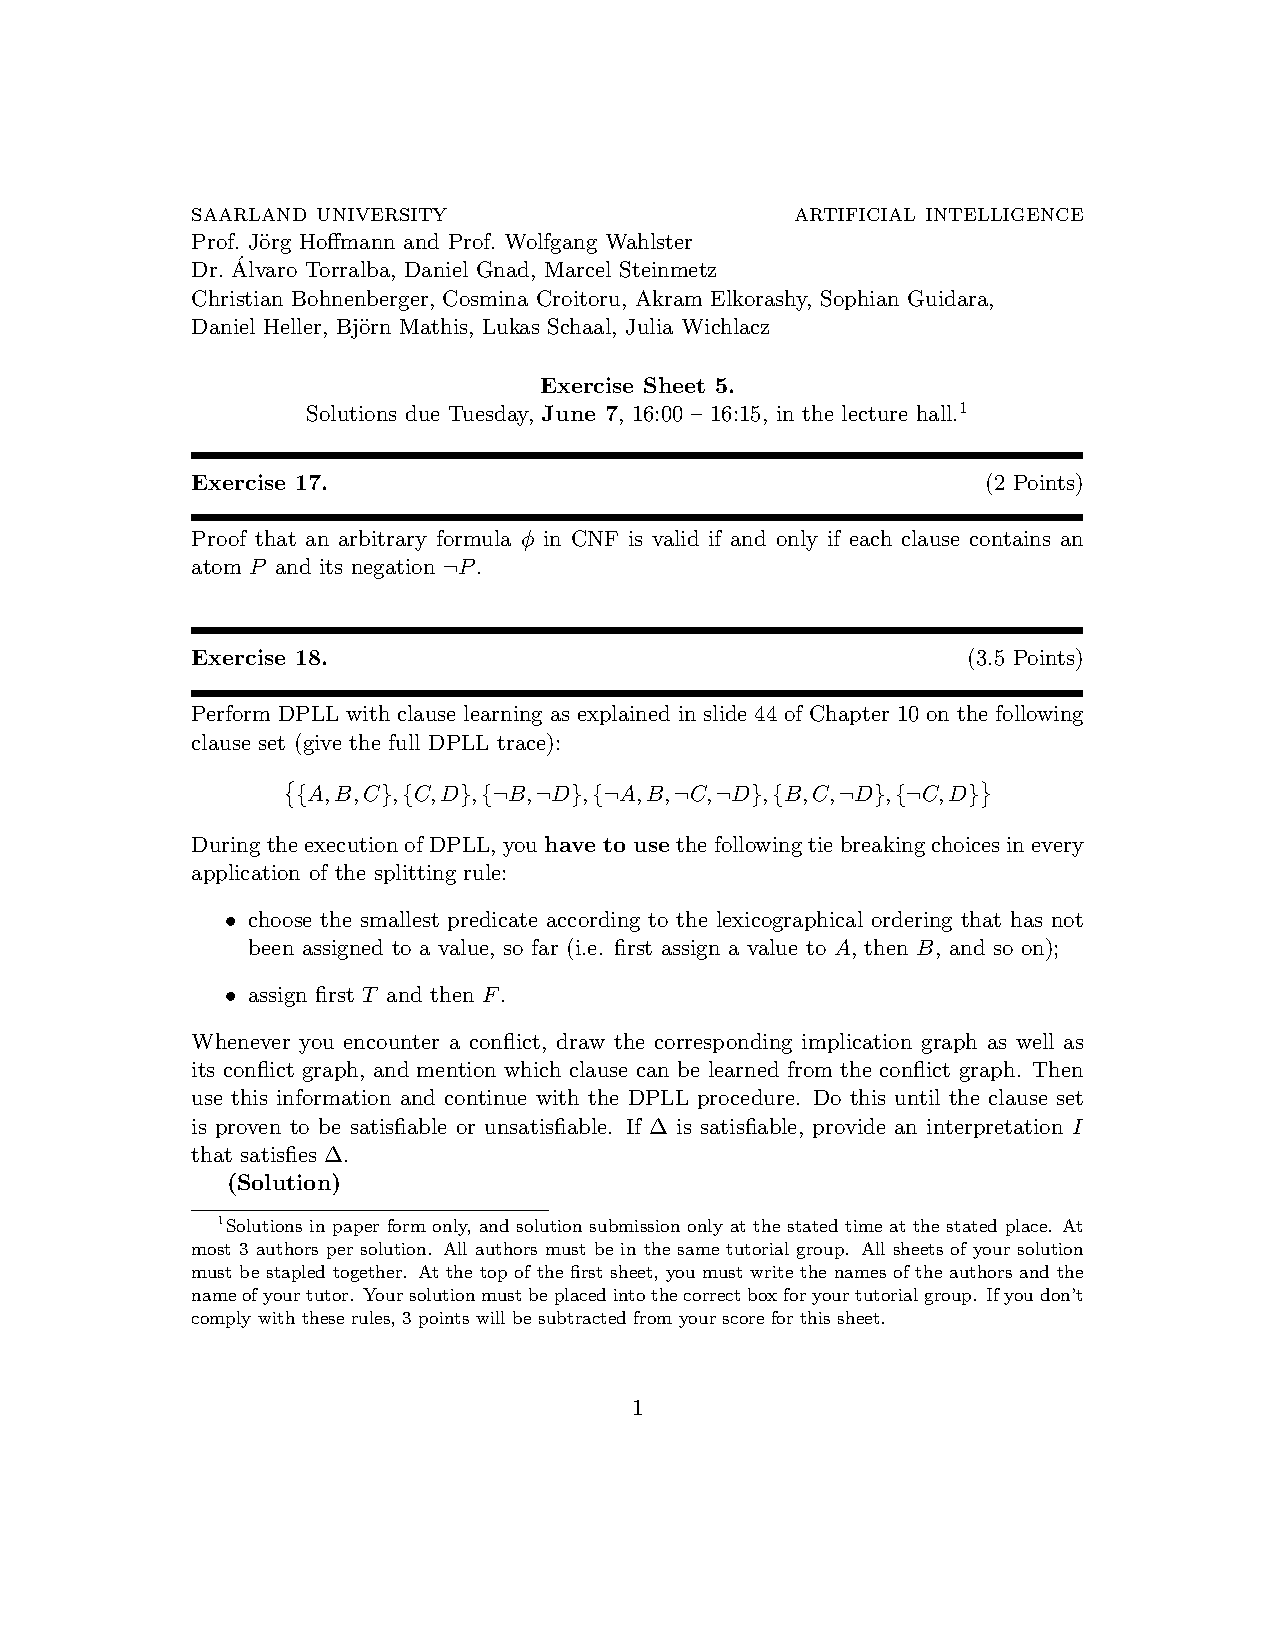
\includepdf[pages=-,nup=2x2]{Old/ai16_sheet05_solution.pdf}
    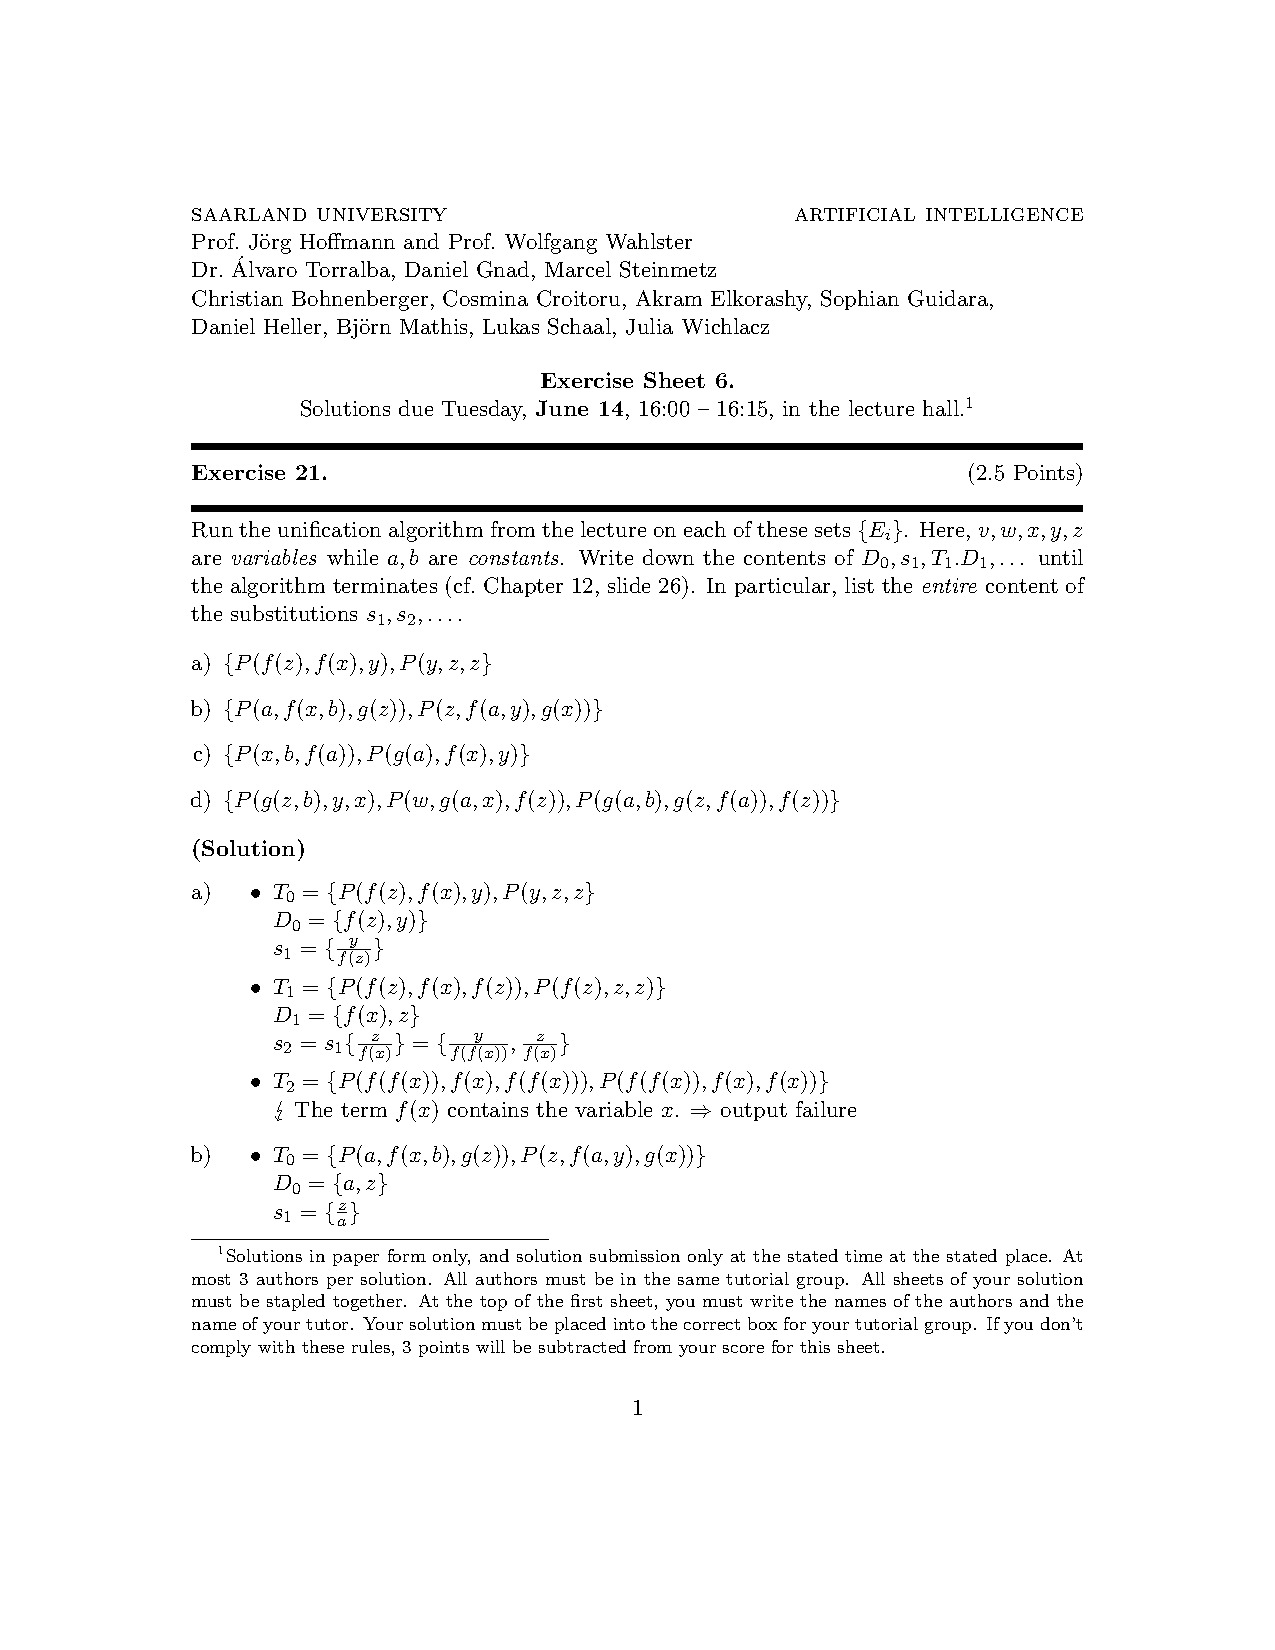
\includepdf[pages=-,nup=2x2]{Old/ai16_sheet06_solution.pdf}
    
    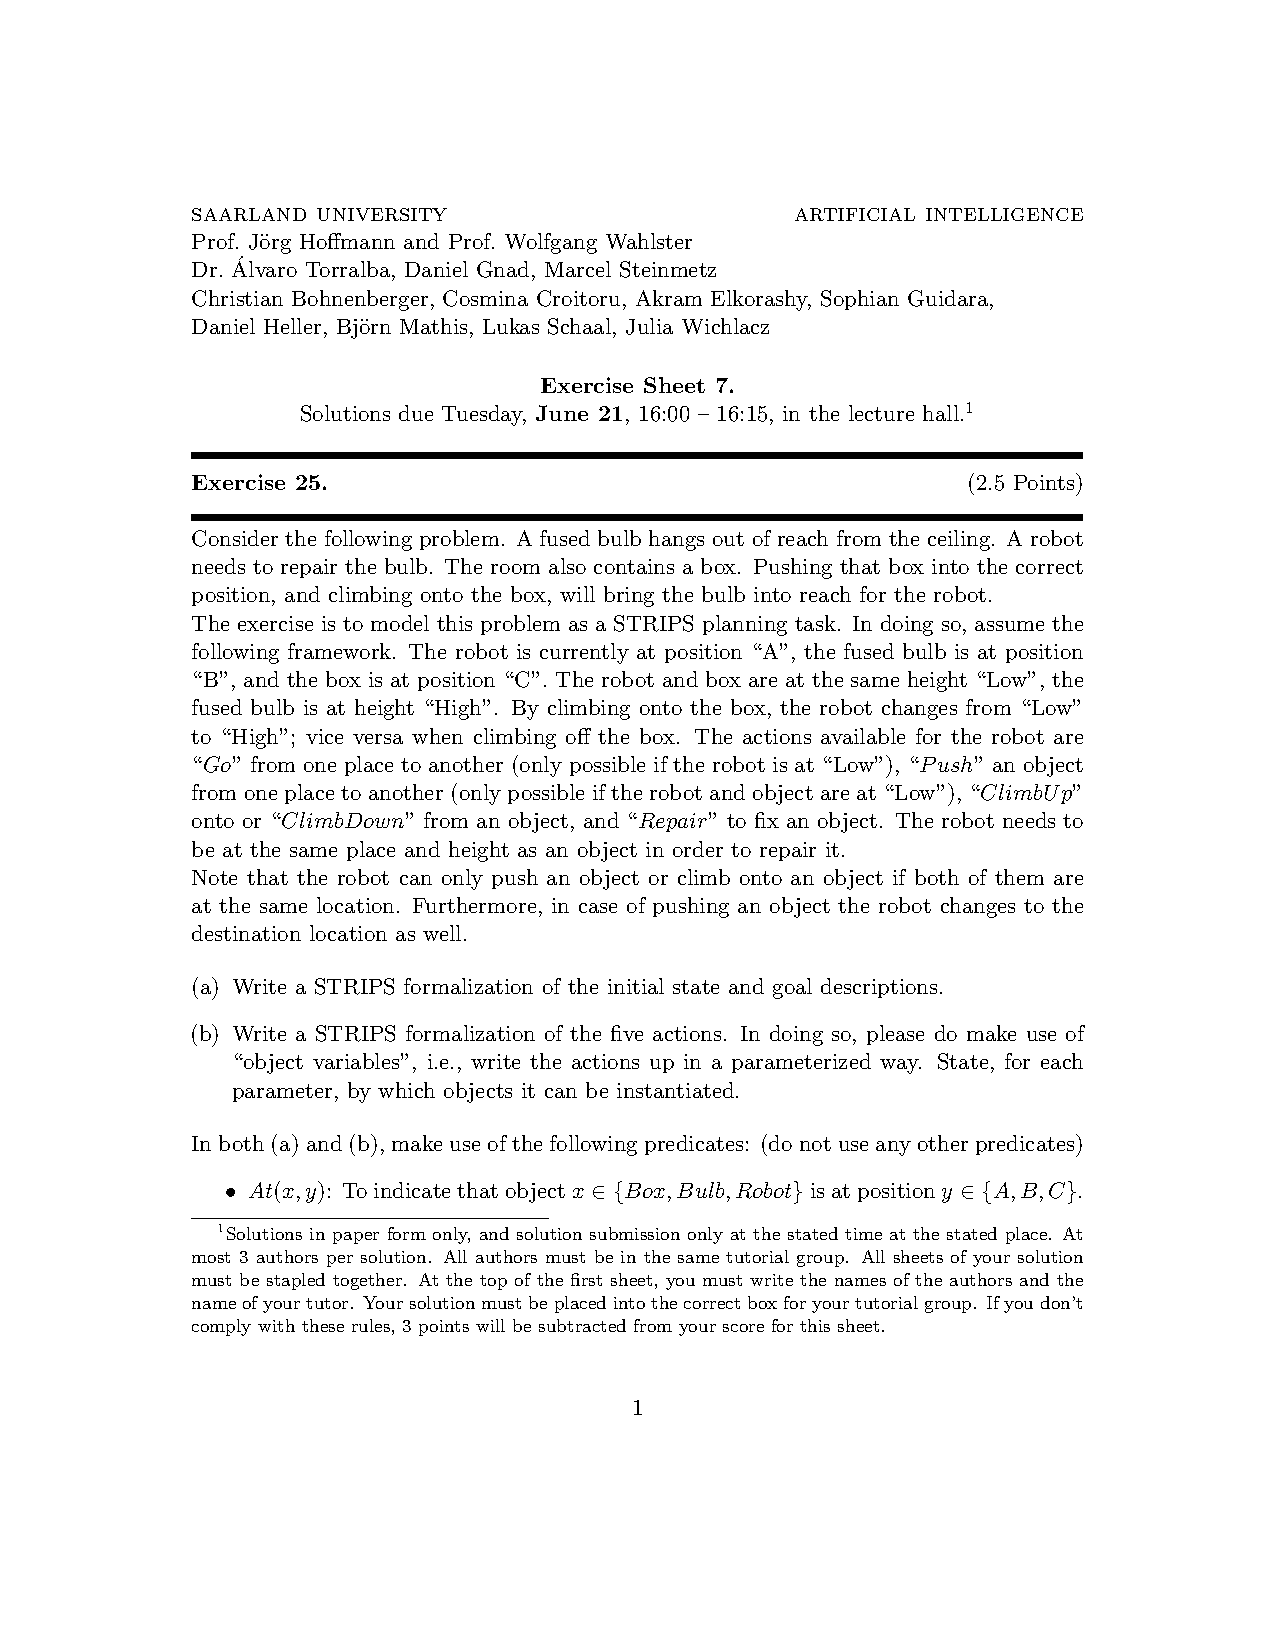
\includepdf[pages=-,nup=2x2]{Old/ai16_sheet07_solution.pdf}
    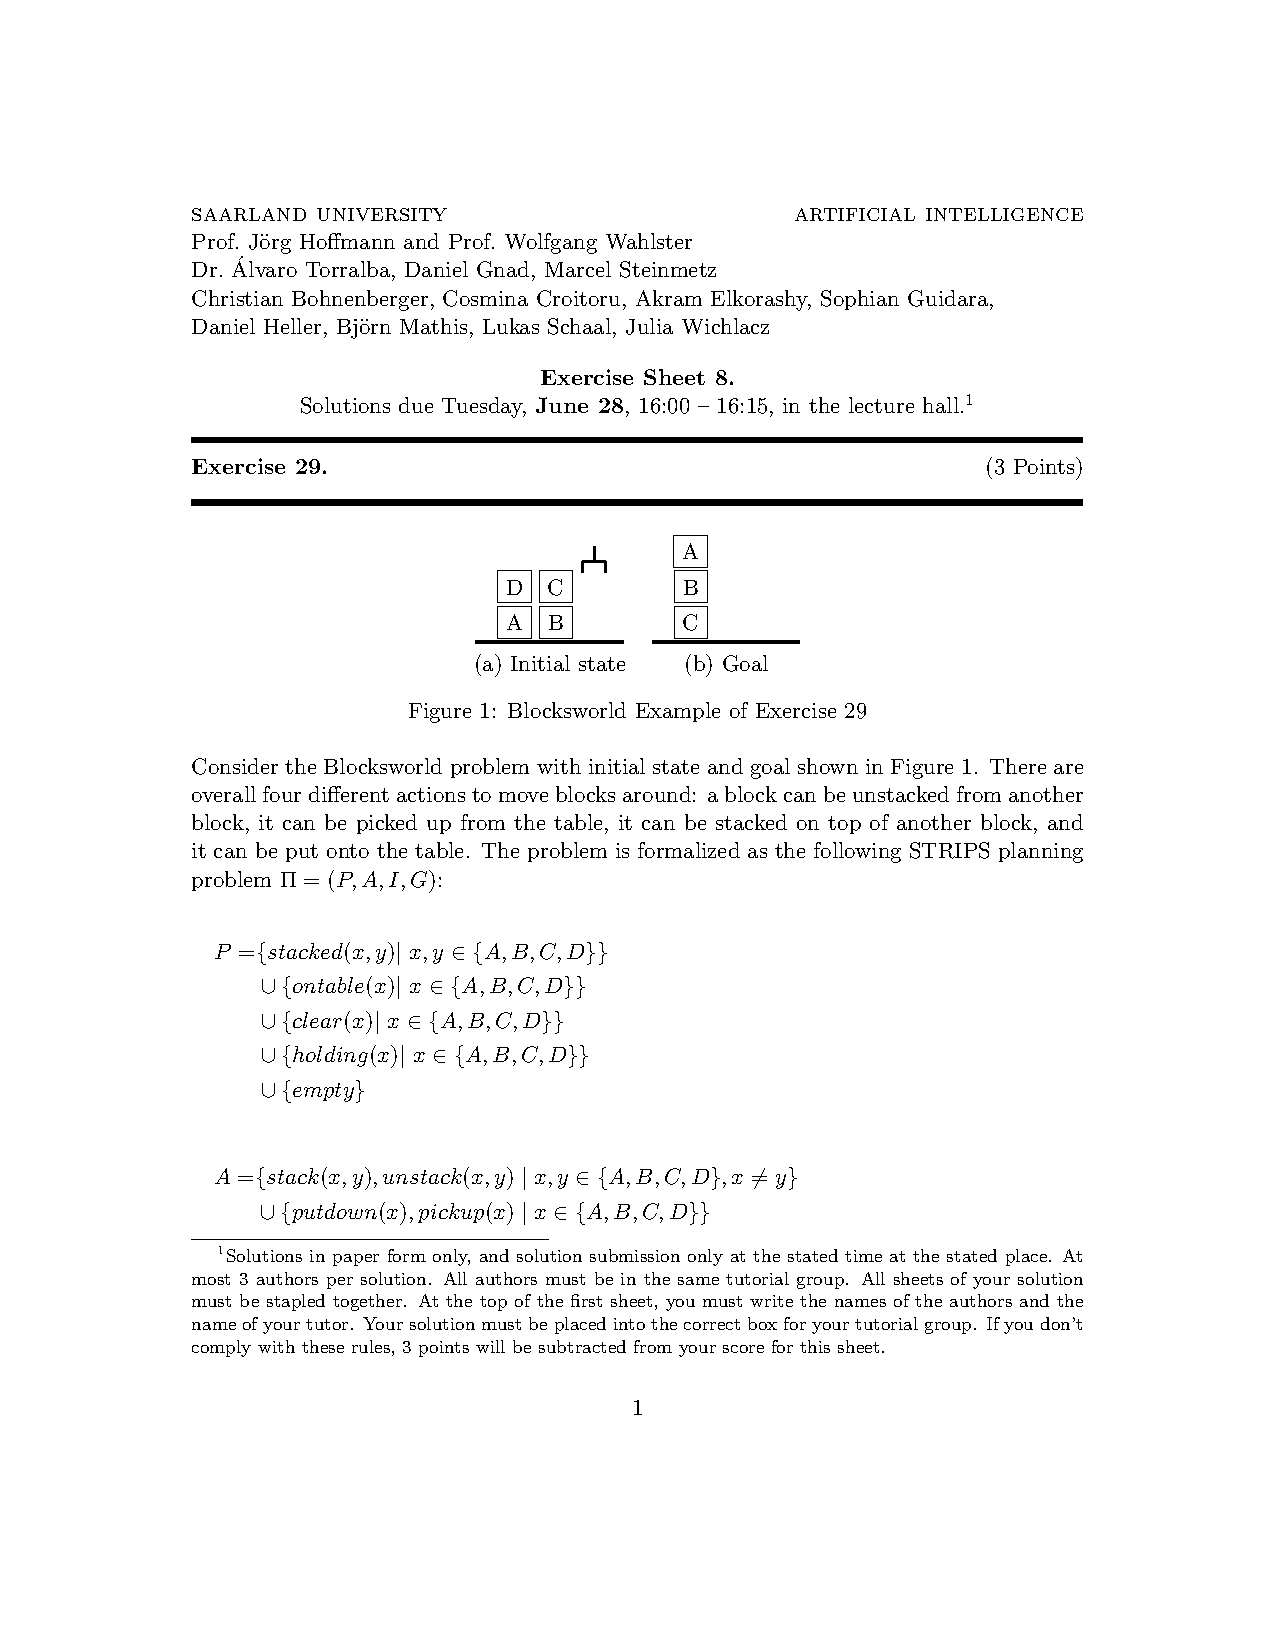
\includepdf[pages=-,nup=2x2]{Old/ai16_sheet08_solution.pdf}
    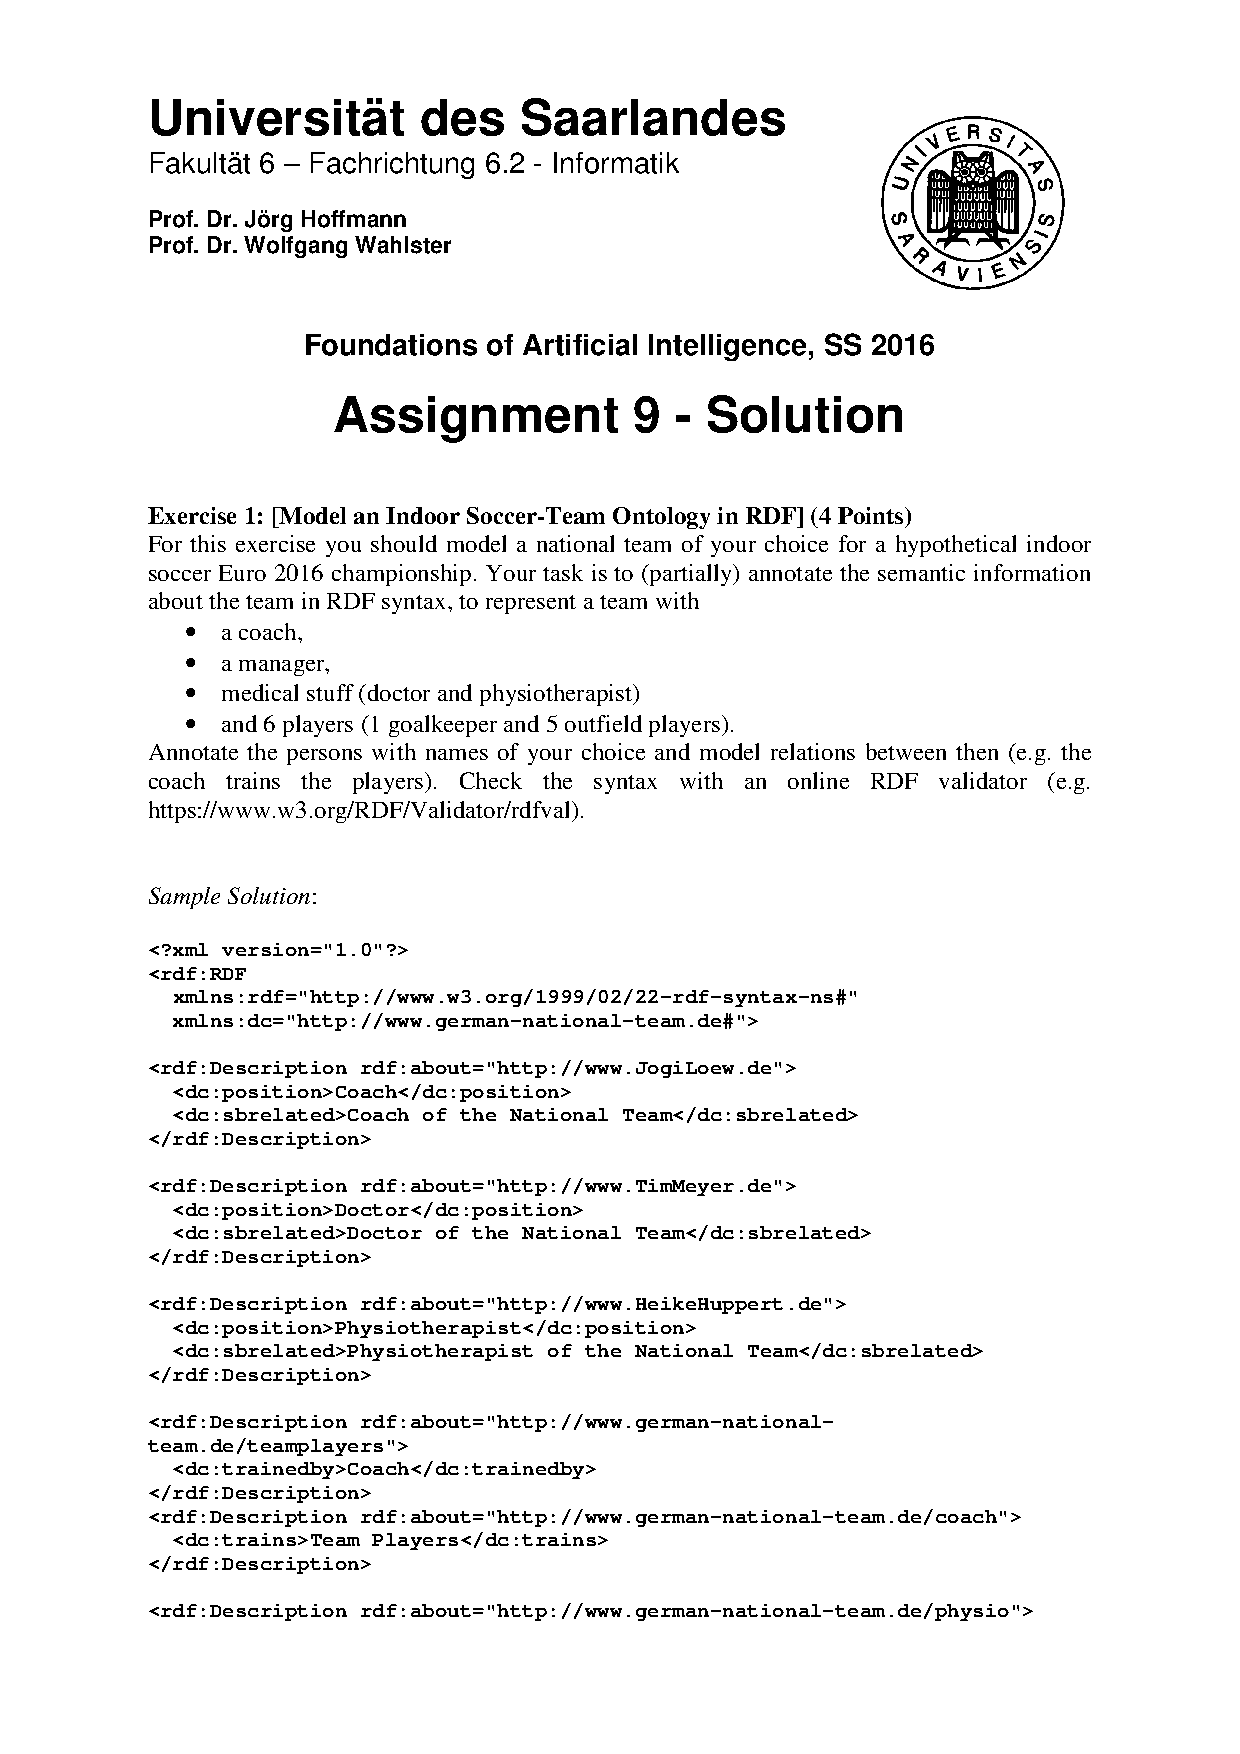
\includepdf[pages=-,nup=2x2]{Old/ai16_sheet09_solution.pdf}
    
    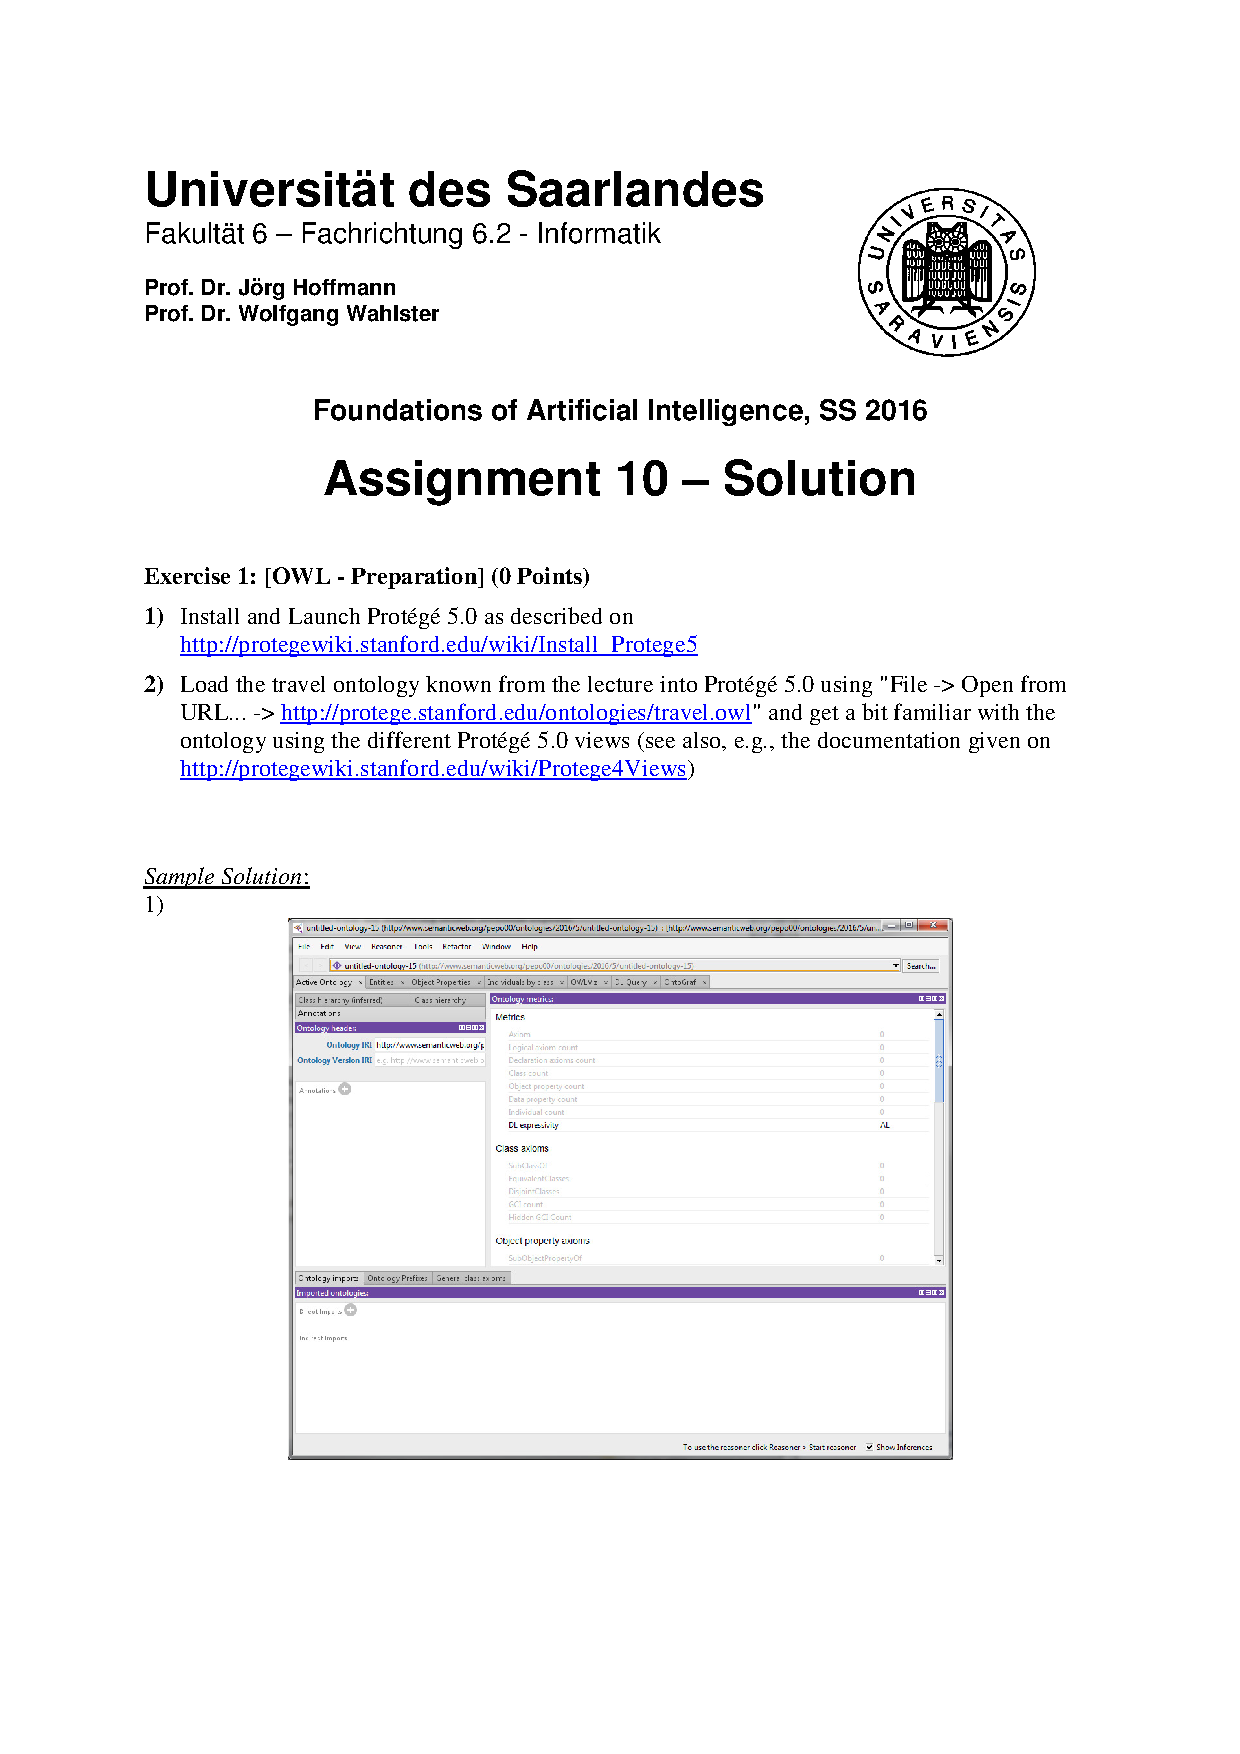
\includepdf[pages=-,nup=2x2]{Old/ai16_sheet10_solution.pdf}

\end{document}
